\documentclass[11pt, fleqn]{article}
\usepackage[english]{babel}

\usepackage[lmargin=1.1in,rmargin=1.1in,bottom=1.3in,top=1.3in,
twoside=False]{geometry}

\usepackage{relsize,xspace}
 \usepackage{xcolor}
 \usepackage{mathtools}
 \usepackage{todonotes}
 \usepackage{comment}
\usepackage{microtype}
\usepackage{amsmath}
\usepackage{amssymb}
\usepackage{amsfonts}
\usepackage{stmaryrd}
\usepackage{bm}
\usepackage{tikz}
\usepackage{refcount}
\usepackage{wrapfig}

\usepackage{marginnote}

\definecolor{sz}{rgb}{0.1,0.2,0.6}
\definecolor{blue}{rgb}{0.1,0.2,0.5}
\definecolor{brown}{rgb}{0.6,0.6,0.2}
%\usepackage[ocgcolorlinks, linkcolor={blue}, citecolor={brown}]{hyperref}
\newcommand{\sebi}[1]{\textcolor{red}{#1}}

\newenvironment{change}[1]
{\begingroup\color{#1}}
{\endgroup}

\usepackage[amsmath,thmmarks,hyperref]{ntheorem}
\usepackage{cleveref}


\crefformat{page}{#2page~#1#3}%
\Crefformat{page}{#2Page~#1#3}%
\crefformat{equation}{#2(#1)#3}%
\Crefformat{equation}{#2(#1)#3}%
\crefformat{figure}{#2Figure~#1#3}%
\Crefformat{figure}{#2Figure~#1#3}%
\crefformat{section}{#2Section~#1#3}
\Crefformat{section}{#2Section~#1#3}
\crefformat{chapter}{#2Chapter~#1#3}
\Crefformat{chapter}{#2Chapter~#1#3}
\crefformat{chapter*}{#2Chapter~#1#3}
\Crefformat{chapter*}{#2Chapter~#1#3}
\crefformat{part}{#2Part~#1#3}
\Crefformat{part}{#2Part~#1#3}
\crefformat{enumi}{#2(#1)#3}
\Crefformat{enumi}{#2(#1)#3}

\usepackage{enumerate}

\usepackage{latexsym}

% BEGIN ntheorem configuration

\theoremnumbering{arabic}
\theoremstyle{plain}
\theoremsymbol{}
\theorembodyfont{\itshape}
\theoremheaderfont{\normalfont\bfseries}
\theoremseparator{.}

\newtheorem{theorem}{Theorem}
\crefformat{theorem}{#2Theorem~#1#3}
\Crefformat{theorem}{#2Theorem~#1#3}
\renewcommand{\setminus}{-}
\newcommand{\newtheoremwithcrefformat}[2]{%
  \newtheorem{#1}[lemma]{#2}%
  \crefformat{#1}{##2\MakeUppercase#1~##1##3}%
  \Crefformat{#1}{##2\MakeUppercase#1~##1##3}%
}
\newcommand{\newseptheoremwithcrefformat}[2]{%
  \newtheorem{#1}{#2}%
  \crefformat{#1}{##2\MakeUppercase#1~##1##3}%
  \Crefformat{#1}{##2\MakeUppercase#1~##1##3}%
}

\newseptheoremwithcrefformat{lemma}{Lemma}
\newtheoremwithcrefformat{proposition}{Proposition}
\newtheoremwithcrefformat{observation}{Observation}
\newtheoremwithcrefformat{conjecture}{Conjecture}
\newtheoremwithcrefformat{corollary}{Corollary}
\newseptheoremwithcrefformat{claim}{Claim}
\newseptheoremwithcrefformat{goal}{Goal}
\theorembodyfont{\upshape}
\newtheoremwithcrefformat{example}{Example}
\newtheoremwithcrefformat{remark}{Remark}
\newseptheoremwithcrefformat{definition}{Definition}

\theoremstyle{nonumberplain}
\theoremheaderfont{\scshape}
\theorembodyfont{\normalfont}
\theoremsymbol{\ensuremath{\square}}
\newtheorem{proof}{Proof}

\theoremsymbol{\ensuremath{\lrcorner}}
\newtheorem{clproof}{Proof}

% END ntheorem configuration

\newcommand{\set}[1]{\{#1\}}
\newcommand{\setof}[2]{\left\{#1 \,\mid\, #2 \right\}}
\renewcommand{\subset}{\subseteq}

%\setlength{\parskip}{0.1cm}
%\setlength{\parindent}{0cm}
%\setlength{\mathindent}{1cm}

\newcommand{\wcol}{\mathrm{wcol}}
\newcommand{\col}{\mathrm{col}}
\newcommand{\adm}{\mathrm{adm}}
\newcommand{\tw}{\mathrm{tw}}
\newcommand{\WReach}{\mathrm{WReach}}
\newcommand{\SReach}{\mathrm{SReach}}
\newcommand{\wcolorder}{\sqsubseteq}
\newcommand{\Oof}{\mathcal{O}}
\newcommand{\CCC}{\mathcal{C}}
\newcommand{\NNN}{\mathcal{N}}
\newcommand{\WWW}{\mathcal{W}}
\newcommand{\DDD}{\mathcal{D}}
\newcommand{\PPP}{\mathcal{P}}
\newcommand{\FFF}{\mathcal{F}}
\newcommand{\GGG}{\mathcal{G}}
\newcommand{\YYY}{\mathcal{Y}}
\newcommand{\nei}{\mathrm{nei}}
\renewcommand{\ker}{\mathrm{ker}}
\newcommand{\core}{\mathrm{core}}

\newcommand{\cutrk}{\mathrm{cutrk}}
\newcommand{\rank}{\mathrm{rank}}
\newcommand{\rw}{\mathrm{rw}}


\newcommand{\grad}{\nabla}
\newcommand{\ds}{\mathbf{ds}}
\newcommand{\cl}{\mathrm{cl}}
\newcommand{\cst}{\alpha}

\newcommand{\fnei}{f_{\nei}}
\newcommand{\fwcol}{f_{\wcol}}
\newcommand{\fker}{f_{\ker}}
\newcommand{\fproj}{f_{\mathrm{proj}}}
\newcommand{\fcl}{f_{\cl}}
\newcommand{\fgrad}{f_{\grad}}
\newcommand{\fpaths}{f_{\mathrm{pth}}}
\newcommand{\fapx}{f_{\mathrm{apx}}}
\newcommand{\fcore}{f_{\mathrm{core}}}
\newcommand{\ffin}{f_{\mathrm{fin}}}

\newcommand\blfootnote[1]{%
  \begingroup
  \renewcommand\thefootnote{}\footnote{#1}%
  \addtocounter{footnote}{-1}%
  \endgroup
}

\newcommand{\suchthat}{ \colon }
\newcommand{\sth}{ \colon }
\newcommand{\ie}{i.e.\@ }
\newcommand{\Pow}{\mathcal{P}}
\newcommand{\N}{\mathbb{N}}
\newcommand{\R}{\mathbb{R}}
\newcommand{\tup}[1]{\bar{#1}}
\renewcommand{\phi}{\varphi}
\renewcommand{\epsilon}{\varepsilon}
\newcommand{\str}{\mathbb}
\newcommand{\strA}{\str{A}}
\newcommand{\strB}{\str{B}}
\newcommand{\FO}{\mathrm{FO}}
\newcommand{\minor}{\preccurlyeq}
\newcommand{\dist}{\mathrm{dist}}
\newcommand{\indx}{\mathrm{index}}
\renewcommand{\mid}{~:~}

\newcommand{\profnum}{\widehat{\nu}}
\newcommand{\projnum}{\mu}
\newcommand{\projprof}{\widehat{\mu}}

\newcommand{\abs}[1]{\ensuremath{\left\lvert#1\right\rvert}}

\newcommand{\im}{\mathrm{im}}
\newcommand{\rg}{\mathrm{rg}}
\newcommand{\from}{\colon}

\renewcommand{\leq}{\leqslant}
\renewcommand{\geq}{\geqslant}
\renewcommand{\le}{\leqslant}
\renewcommand{\ge}{\geqslant}

\hypersetup{ocgcolorlinks=true,colorlinks=true,linkcolor={blue}, citecolor={brown}}

\newcounter{aux}

\title{On the number of types in sparse graphs
\thanks{
The work of M.\ Pilipczuk and S.\ Siebertz is supported by the National Science Centre of 
Poland via POLONEZ grant agreement UMO-2015/19/P/ST6/03998, 
which has received funding from the European Union's Horizon 2020 research and 
innovation programme (Marie Sk\l odowska-Curie grant agreement No.\ 665778).
The work of Sz.~Toru{\'n}czyk is supported by the National Science Centre of Poland grant 2016/21/D/ST6/01485.
M. Pilipczuk is supported by the Foundation for Polish Science (FNP) via the START stipend programme.
}}

\author{
Micha\l~Pilipczuk \qquad
\qquad Sebastian Siebertz
\qquad Szymon Toru{\'n}czyk\\[0.3cm]
Institute of Informatics, University of Warsaw, Poland\\[0.1cm]
\texttt{\{michal.pilipczuk,siebertz,szymtor\}@mimuw.edu.pl}}

\begin{document}

\maketitle
We prove that for every nowhere dense class of graphs $\CCC$, as
defined by Ne\v set\v ril and Ossona de
Mendez~\cite{nevsetvril2010first,nevsetvril2011nowhere}, and for every
first order formula $\phi(\tup x,\tup y)$, whenever one draws a graph
$G\in \CCC$ and a subset of its vertices $A$, the number of subsets of
$A^{|\tup y|}$ that are of the form $\set{\tup v\in A^{|\tup y|}\,
\colon\, G\models\phi(\bar u,\tup v)}$ for some valuation~$\tup u$ of
$\tup x$ in $G$ is bounded by $\Oof(|A|^{|\tup x|+\epsilon})$, for
every $\epsilon>0$. This provides optimal bounds on the VC-density of
first-order definable set systems in nowhere dense graph classes.
%
We also give two new proofs of upper bounds on quantities in nowhere
dense classes that are relevant for their logical treatment. First, we
provide a new proof of the fact that nowhere dense classes are
uniformly quasi-wide, implying explicit, polynomial upper bounds on
the functions relating the two notions. Second, we give a new
combinatorial proof of the result of Adler and
Adler~\cite{adler2014interpreting} stating that every nowhere dense
class of graphs is stable. In contrast to the previous proofs of the
above results, our proofs are completely finitistic and constructive,
and yield explicit and computable upper bounds on quantities related
to uniform quasi-wideness (margins) and stability (ladder indices).

\begin{picture}(0,0) \put(397,-217)
{\hbox{\includegraphics[scale=0.25]{flag_bw.jpg}}} \end{picture} 
\vspace{-0.8cm}

%\section{Introduction}

Nowhere dense classes of graphs were introduced 
by Nešetřil and Ossona de 
Mendez~\cite{nevsetvril2010first,nevsetvril2011nowhere} as a very 
general model
for uniform sparseness of graphs. These classes generalize many 
familiar classes of sparse graphs, such as planar graphs, graphs 
of bounded treewidth,  graphs of bounded degree, and, in fact, 
all classes that exclude a fixed 
topological minor.
The concept of nowhere denseness
turns out to be very robust as witnessed by the fact that it is equivalent 
to multiple other concepts studied in different areas of mathematics. 
One can equivalently characterize nowhere dense graph classes 
by bounds on the density of shallow (topological)
minors~\cite{nevsetvril2010first,nevsetvril2011nowhere},
quasi-wideness~\cite{nevsetvril2011nowhere} (a notion introduced by
Dawar~\cite{dawar2010homomorphism} in his study of homomorphism
preservation properties), low tree-depth
colorings~\cite{nevsetvril2008grad}, generalized coloring
numbers~\cite{zhu2009coloring}, sparse neighborhood
covers~\cite{GroheKRSS15,grohe2014deciding}, by a game called the
splitter game~\cite{grohe2014deciding} and by the model-theoretic
concepts of stability and independence~\cite{adler2014interpreting}.
For a broader discussion on the graph theoretic sparsity we refer to the book
of Ne\v{s}et\v{r}il and Ossona de Mendez~\cite{sparsity}.

These alternative characterizations have been very useful in 
the design of efficient algorithms. For instance, 
the {\sc{Subgraph Isomorphism}} and {\sc{Homomorphism}} problems 
are fixed-parameter tractable on any nowhere dense
class, parameterized by the size of the pattern graph~\cite{nevsetvril2010first}
and so is the {\sc Distance-$r$ Dominating Set} problem, parameterized
by the size of the solution~\cite{DawarK09}. In fact, 
the {\sc Distance-$r$ Dominating Set} problem admits
polynomial kernels~\cite{siebertz2016polynomial} and even 
almost linear kernels on nowhere dense classes of 
graphs~\cite{eickmeyer2016neighborhood}
(see also~\cite{drange2016kernelization} for the case $r=1$). 
It was shown in~\cite{grohe2014deciding}
that every first-order definable problem can be decided in
almost linear time on any nowhere dense graph class.

It is a natural question to ask for the most general classes of graphs
which admit efficient solutions for certain problems, or to 
classify them into tractable and intractable classes. It was shown 
that for the first-order model-checking problem~\cite{dvovrak2013testing} and for
the {\sc Distance-$r$ Dominating Set} problem~\cite{drange2016kernelization} 
the dividing line for algorithmic tractability 
on subgraph closed classes of graphs is exactly between the
nowhere dense and somewhere dense graph classes. 

\smallskip

In (infinite) model theory, we are following a different classification program. We 
want to count the number and classify the models of a complete theory. According
to the upward L\"ownheim-Skolem theorem, every theory $T$ with an infinite model has
models of arbitrary infinite cardinalities (larger then the size of the language). We 
now ask for any fixed infinite cardinal~$\kappa$ how many models of cardinality 
$\kappa$ the theory $T$ can have (up to isomorphism). Note that the number of
models of cardinality $\kappa$ must lie between $1$ and $2^\kappa$ for all infinite cardinals $\kappa$ 
bigger than the cardinality of the language. By a result of 
Morley~\cite{morley1965categoricity}, if $T$ is a countable
theory which has only one model of cardinality $\kappa$ for some uncountable $\kappa$, 
then $T$ has only one model for all uncountable cardinals; a result which 
is often considered the starting point of modern model theory. In his famous classification
project~\cite{shelah1990classification}, Shelah essentially provided a complete
classification for all countable theories (the classification was completed 
in~\cite{hart2000uncountable}). Shelah identified several dividing lines and showed that
all theories on the non-structure side of the dividing line have $2^\kappa$ models
of cardinality $\kappa$. On
the structure side he showed that there are only few models whose isomorphism 
types can be described by small invariants. One of the most important dividing 
lines is \emph{stability}. Very roughly, if a theory is not stable then its models 
are too many and too complicated to classify, while this may be possible if the theory is stable, 
especially if the theory is \emph{superstable} or \emph{totally transcendental}.

Finite model theory is the study of the expressive power 
of logics on the class of finite structures. Many theorems and 
methods of classical model theory fail when only finite structures 
are considered. These include the compactness theorem, the completeness 
theorem and various interpolation and preservation theorems.
On the other hand, quite different questions, which often come from
computer science, in particular questions from complexity theory and database
theory, are interesting in finite model theory. Hence, instead of focusing 
on negative results, much work has been invested in finding 
subclasses of the class of all finite structures that may be better behaved.
Surprisingly, it turns out that particularly classes which are 
algorithmically well-behaved turn out to have good model-theoretic 
properties. The two prime examples in our context are the result of 
Dawar~\cite{dawar2010homomorphism}, who introduced the notion of
quasi-wideness and proved any quasi-wide class that is closed under taking substructures
and disjoint unions has the homomorphism preservation property. It was 
later proved by Ne\v{s}et\v{r}il and Ossona de Mendez that 
the notions of uniform quasi-wideness and nowhere denseness coincide for 
graphs~\cite{nevsetvril2011nowhere}. The second result is by 
Adler and Adler~\cite{adler2014interpreting}, who observed that 
nowhere denseness essentially corresponds to the stability theoretic notion 
of \emph{superflatness} introduced by Podewski and 
Ziegler in~\cite{podewski1978stable}. In fact, Adler and Adler observed 
that on subgraph closed classes of graphs, the notions of nowhere denseness, 
stability and the non-independence property (NIP) are equivalent. 
Before we can give an 
overview of some of the techniques that can be brought down from 
the uncountable to the finite and state our contributions, we need some
definitions. 

\begin{definition}
Let $T$ be a complete theory in a first-order language $L$. Let 
$\phi(\tup{x},\tup{y})$ be an $L$-formula with the free variables
divided into two groups $\tup{x}, \tup{y}$. An \emph{$n$-ladder}
for $\phi$ is a sequence $(\tup{a}_0,\ldots, \tup{a}_{n-1},
\tup{b}_0,\ldots, \tup{b}_{n-1})$ of tuples in some model $\strA$
of $T$, such that
\[\text{for all $0\leq i,j<n$, }\strA\models\phi(\tup{a}_i,\tup{b}_j)\Longleftrightarrow i\leq j. \]
A formula $\phi$ is \emph{stable} (for $T$, or for $\strA$) if there is 
some $n\in \N$ such that no $n$-ladder for $\phi$ exists, otherwise, 
$\phi$ is \emph{unstable}. The least such $n$ is the \emph{ladder index}
of $\phi(\tup{x},\tup{y})$ (which may depend on the way we split the
variables). A class $\CCC$ of structures is \emph{stable} if the ladder index
of every formula~$\phi$ is bounded by a constant $n=n(\CCC,\phi)$
on all $\strA\in \CCC$.
\end{definition}

We remark that a formula with ladder index $n$ is said to have the
$n$-order property in~\cite{adler2014interpreting} and~\cite{ensley1996finite}.
We follow the notation of the textbook~\cite{hodges1993model} and remark
that it is easy to see that a class $\CCC$ is stable if and only if there is no 
formula $\psi(\tup{x},\tup{y})$ such that for every $n\in \N$
there exist a structure $\strA\in \CCC$ and tuples $\tup{a}_0,\ldots, \tup{a}_{n-1}$
of elements of $\strA$ such that $\strA\models\psi(\tup{a}_i,\tup{a}_j)\Leftrightarrow i<j$,
that is, $\psi$ orders the tuples linearly. 

The first application of stability theory concerns the existence of long
indiscernible sequences. If $\tup{a}=(a_0,\ldots)$ is a non-repeating sequence of elements of $\strA$, we write \[[\tup{a}]^k\coloneqq \{\tup{b}=(a_{i_1},\ldots, a_{i_k}) \sth 0\leq i_1<\ldots <i_k\}\] for the set of of all subsequences
of $\tup{a}$ of length $k$. When we speak of a subsequence $\tup{a}'$
of a sequence $\tup{a}$, we always mean an increasing subsequence. 

\begin{definition}
Let $\tup{a}=(a_0,\ldots)$ be a non-repeating sequence of elements of $\strA$.
Let $f$ be a map with domain $[\tup{a}]^k$. A subsequence $\tup{a}'$ 
of $\tup{a}$ is \emph{$f$-indiscernible} if for any two 
subsequences $\tup{v},\tup{w}\in [\tup{a}']^k$ 
it holds that $f(\tup{w})=f(\tup{w})$.

If $\Phi$ is a set of formulas of the form $\phi(x_0,\ldots, x_{k-1})$, 
we say that $\tup{a}'$ 
is \emph{$\Phi$-indiscernible} (in a structure $\strA$)
if for every $\phi\in \Phi$ and any two 
subsequences $\tup{v},\tup{w}\in [\tup{a}]^k$ it
holds that $\strA\models\phi(\tup{a})\Leftrightarrow\strA\models\phi(\tup{b})$. 
\end{definition}

%We often identify ordered sets with sequences of elements. 
%A sequence $(a_1,\ldots, a_\ell)$ of elements of~$\strA$ is
%\emph{$\Phi$-indiscernible} if for every formula
%$\phi(x_1,\ldots, x_k)\in \Phi$ with $k$ free variables and any two
%increasing sequences
%$1\leq i_1<\ldots <i_k\leq \ell, 1\leq j_1< \ldots< j_k\leq \ell$ of
%integers, it holds that
%\[\strA\models\phi(a_{i_1},\ldots, a_{i_k})\Leftrightarrow \strA\models\phi(a_{j_1},
%\ldots, a_{j_k}).\]

Results about the existence of indiscernible sequences are known as 
\emph{partition theorems}, because the map $f$ induces a partition
on the set $[\tup{a}]^k$ (which can be identified with the ordered 
set $A=\{a_0,\ldots\}$). Partitioning theorems play an important role in 
combinatorics and graph theory, and also in stability theory. The 
crucial distinction in stability theory is between \emph{Ramsey type 
theorems}, which hold
for reason of cardinality alone, and \emph{stability type theorems},
which take into account the underlying structure (theory). The following
theorem shows that we need the sequence $A$ to be only polynomially larger
than the indiscernible sequence $B$ we are aiming at if we are in a stable theory. 
It is easy to make the theorem algorithmic, see 
e.g.~\cite{siebertz2016polynomial}. 

\begin{theorem}[Malliaris and Shelah~\cite{malliaris2014regularity}, Theorem 3.5, Item (2)]\label{thm:malshelah}
  Let  $\Delta$ be a finite
  set of stable first-order formulas.  There is a polynomial $p(x)$ such that
  for all $\strA\in \CCC$, every positive integer $m$ and every non-repeating sequence
  $\tup{a}=(a_0,\ldots, a_{\ell-1})$ of elements of $\strA$ of length $\ell=p(m)$, there
  exists a sub-sequence $\tup{a}'$ of
  $\tup{a}$ of length $m$ which is
  $\Delta$-indiscernible.
\end{theorem}

Another perspective on stability theory is to see it as a way of 
classifying definable sets in a structure and describing the interaction 
between definable sets. For this, we need the notion of types. 

\begin{definition}
Let $\Delta$ be a set of $L$-formulas, let $\strA$ be an $L$-structure and let
$A$ be a set of elements of $\strA$. Let $a$ be an element of $\strA$. The 
\emph{$\Delta$-type of~$a$ in $\strA$ over the parameters $A$} is the set
\begin{align*}
  \mathrm{tp}_\Delta(\strA, A, a) & \coloneqq  \{ \phi(x_1,a_1,\ldots, a_k)  : &\\
  &  \hspace{3.1cm}
                                \phi(x_1,y_1,\ldots, y_k)\in \Delta,
                                a_1,\ldots, a_k\in A,
                                \strA\models\phi(a,a_1,\ldots, a_k)\}.
\end{align*}
The set of \emph{$\Delta$-types realised} in $\strA$ over $A$ is the set
$S_\Delta(\strA,A) \coloneqq \{ \mathrm{tp}_\Delta(\strA, A, a) \sth a$ element of $\strA\}$.
\end{definition}

We usually assume that $\Delta$ is closed under negations. 
The number of realised types over a parameter set of cardinality
$\kappa$ can be anything between $0$ and $\abs{\Delta}\cdot 2^\kappa$. 
Shelah proved that
in a \emph{dependent} theory the number of realised types will always be
at most polynomial, and also this theorem carries over to the finite. 

\begin{definition}
Let $T$ be a complete theory in a first-order language $L$. Let 
$\phi(\tup{x},\tup{y})$ be an $L$-formula with the free variables
divided into two groups $\tup{x}, \tup{y}$. The formula $\phi$ has
the \emph{$n$-independence property} if in some model $\strA$
of $T$, there are tuples $\tup{a}_0,\ldots, \tup{a}_{n-1}$ and
$\tup{b}_J$ for $J\subseteq \{0,\ldots, n-1\}$ such that
\[\strA\models\phi(\tup{a}_i,\tup{b}_J)\Longleftrightarrow i\in J. \]
A formula $\phi$ is \emph{dependent} (for $T$, or for $\strA$) if there is 
some $n\in \N$ such that $\phi$ does not have the $n$-independence property. 
A class $\CCC$ of structures is \emph{dependent} or has the \emph{non-independence property}, 
short \emph{NIP}, if for every formula~$\phi$ there is constant $n=n(\CCC,\phi)$
such that $\phi$ does not have the $n$-independence property on all $\strA\in \CCC$.
\end{definition}

\begin{theorem}[\cite{shelah1990classification}, Theorem II.4.10(4) and II.4.11(4)]
Let $\Delta$ be a finite set of first-order formulas which are 
dependent on $\strA$. Then there exists a positive integer $k$ such that 
for any set~$A$ of elements of $\strA$ with $\abs{A}\geq 2$ it holds that
$\abs{S_\Delta(\strA,A)}\leq \abs{A}^k$. 
\end{theorem}

The independence property of a formula can be understood as its 
\emph{VC-dimension}~\cite{vapnik2015uniform,laskowski1992vapnik}, 
a concept with many applications in computational
learning theory, see e.g.~\cite{}. 

We now come to the definition of nowhere dense classes, which is based
on excluded bounded-depth minors. 

\begin{definition}
A {\em{minor model}} of a graph $H$ in $G$ is a family $(I_u)_{u\in V(H)}$ of pairwise vertex-disjoint connected subgraphs of $G$
such that whenever $uv$ is an edge in~$H$, there are $u'\in I_u$ and $v'\in I_v$ for which $u'v'$ 
is an edge in $G$.
The graph $H$ is a {\em{depth-$r$ minor}} of $G$, denoted $H\minor_rG$, if there is a minor model
$(I_u)_{u\in V(H)}$ of~$H$ in $G$ such that each subgraph $I_u$ has radius at most $r$.

A graph $H$ is a \emph{topological minor} of a graph $G$ if there is a
function~$\delta$ mapping vertices $v\in V(H)$ to vertices of $V(G)$ and 
edges $e\in E(H)$ to directed paths in $G$ such that 
$\delta(v)\neq \delta(u)$ for all distinct $u,v\in V(H)$, and 
if $e=(u,v)\in E(H)$, then $\delta(e)$ is a path from 
$\delta(u)$ to $\delta(v)$ in~$G$ which is internally vertex disjoint from all 
$\delta(e')$ with $e'\in E(H)$, $e'\neq e$. 
For $r\geq 0$, $H$ is a \emph{topological depth-$r$ minor} of $G$, 
written $H\minor_r^tG$, if it is a topological minor and all paths~$\delta(e)$
have length at most $2r$. If all paths~$\delta(e)$ have length exactly
$r$, we say that $G$ contains an \emph{$r$-subdivision} of $H$ (as a 
subgraph). 
\end{definition}

\begin{definition}
A class $\CCC$ of graphs is \emph{nowhere dense} if there is a function 
$f:\N\rightarrow \N$ such that for all $r\in \N$ it holds that $K_{f(r)}\not\minor_r G$
for all $G\in \CCC$. 
\end{definition}

Equivalently, a 
class $\CCC$ of graphs is nowhere dense if there is a function 
$g:\N\rightarrow \N$ such that for all $r\in \N$ it holds that 
$K_{g(r)}\not\minor_r^t G$ for all $G\in \CCC$, or that the
$r$-subdivision of $K_{g(r)}$ is not a subgraph of all $G\in \CCC$. 
The latter is in fact the definition of \emph{superflat classes of graphs}
(for classes of finite and infinite graphs), 
given by Podewski and Zieger~\cite{podewski1978stable}, who also
proved that superflat classes of graphs are stable. 
The notion of uniform
quasi-wideness introduced by Dawar~\cite{dawar2010homomorphism}
can be seen as a finite analogue of the property 
$(\ast)$ introduced by Podewski and Ziegler. 

\begin{definition}
A set $B\subseteq V(G)$ is called {\em{$r$-independent}} in $G$ if for all
distinct $u,v\in B$ we have $\dist_G(u,v)>r$.
A class $\CCC$ of graphs is \emph{uniformly quasi-wide} if there are
functions $N\colon \N\times\N\rightarrow \N$ and $s:\N\rightarrow \N$ such
that for all $r,m\in \N$ and all subsets $A\subseteq V(G)$ for
$G\in \CCC$ of size $\abs{A}\geq N(r,m)$ there is a set
$S\subseteq V(G)$ of size $\abs{S}\leq s(r)$ and a set
$B\subseteq A\setminus S$ of size $\abs{B}\geq m$ which is $r$-independent in
$G-S$. 
\end{definition}

As shown by Ne\v{s}et\v{r}il and Ossona de Mendez~\cite{nevsetvril2010first},
a class $\CCC$ of graphs is nowhere dense if and only if it
is uniformly quasi-wide.

\paragraph{Our contributions.} In this work we revisit the 
connections between nowhere denseness, quasi-wideness and
stability. 

Our first result is the presentation of a new proof of 
Ne\v{s}et\v{r}il and Ossona de Mendez's result~\cite{nevsetvril2010first},
that a class $\CCC$ of graphs is nowhere dense if and only if it
is uniformly quasi-wide. The proof of Ne\v{s}et\v{r}il 
and Ossona de Mendez goes back to a construction
of Kreidler and Seese~\cite{kreidler1998monadic} (see also Atserias et al.~\cite{atserias2006preservation}), 
and uses iterated Ramsey arguments. Hence the original bounds on 
the function $N$ are huge. Recently, 
it was proved that we may always choose $N$ to be a polynomial 
function~\cite{siebertz2016polynomial}. The degree of the polynomial 
in~\cite{siebertz2016polynomial} was  not specified, its existence 
depends on Adler and Adler's result that nowhere dense classes of graphs
are stable and hence every fixed formula has bounded ladder index 
on every nowhere dense class of graphs. We give a new construction 
which is considerably simpler than that of~\cite{siebertz2016polynomial}
and which gives explicit bounds on the degree of the polynomial. 
We prove the following theorem. 

\begin{theorem}\label{thm:new-uqw}
Let $G$ be a graph such that $K_t\not\minor_{r+2} G$. 
If $A\subseteq V(G)$ of size $\Omega(m^{(6t+3)^{t+r}})$, then we can find a set
$S\subseteq V(G)$ of size $|S|\leq t$ and a set $B\subseteq A\setminus S$ 
of size $|B|\geq m$ which is $r$-independent in $G-S$.  
\end{theorem}

We prove \cref{thm:new-uqw} in \cref{sec:uqw}. We want to highlight
that even though our methods are the methods from stability theory, 
we use only very simple graph theoretic notions. In particular, the
proof can easily be turned into an efficient algorithm which does not
call a model-checking algorithm as a subroutine. 

\bigskip
Podewski and Ziegler's proof that flat graphs are stable uses an 
infinite Ramsey argument. Based on Gaifman's Locality Theorem for
first-order logic~\cite{gaifman1982local}, we give a combinatorial 
proof that every first-order formula has finite ladder index on every
nowhere dense class of graphs. Our proof gives explicit bounds for the
ladder indices of formulas. 

\begin{theorem}\label{thm:new-stable}
Let $\phi(x_1,\ldots, x_k)$ be a formula of quantifer rank $q$. 
Let $G$ be a graph such that $K_t\not\minor_{2^{q+k}} G$. Then 
The ladder index of $\phi$ on $G$ is at most $x$. 
\end{theorem}

We prove \cref{thm:new-stable} in \cref{sec:stable}. 

\bigskip

Finally, we again consider the formula stating that the distance
between two elements is at most $r$. 
We observe that an argument of Bousquet and 
Thomasse\'e~\cite{BousquetT15} can be slightly modified to prove that 
the VC-dimension of the $r$-power graph $G^r$ of a graph $G$
with $K_t\not\minor_r G$ is bounded by $t-1$.

\begin{theorem}\label{thm:new-vc}
Let $G$ be a graph such that $K_t\not\minor_r G$. Then the
VC-dimension of the $r$-power graph~$G^r$ is bounded by $t-1$. 
\end{theorem}

We prove \cref{thm:new-vc} in \cref{sec:vc}. 

\section{Introduction}\label{sec:intro}

Nowhere dense classes of graphs were introduced 
by Ne\v set\v ril and Ossona de 
Mendez~\cite{nevsetvril2010first,nevsetvril2011nowhere} as a very 
general model
capturing uniform sparseness of graphs. These classes generalize many 
familiar classes of sparse graphs, such as planar graphs, graphs 
of bounded treewidth,  graphs of bounded degree, and, in fact, 
all classes that exclude a fixed 
topological minor.
Formally, a class $\CCC$ of graphs is {\em{nowhere dense}} if there is a function $t\colon \N\to \N$ such that for every $r\in \N$, no graph $G$ in~$\CCC$ contains the clique $K_{t(r)}$ on $t(r)$ vertices  as  {\em{depth-$r$ minor}},
i.e., as a subgraph of a graph obtained from $G$ by contracting mutually disjoint  subgraphs of radius at most $r$ to single vertices.
Classes of bounded expansion~\cite{nevsetvril2008grad} 
are important subclasses 
of nowhere dense graph classes which are defined by the existence of a bound of 
the edge density of all depth-$r$ minors of graphs in the class, for every fixed $r$.


The concept of nowhere denseness
turns out to be very robust, as witnessed by the fact that it is equivalent 
to multiple other concepts studied in different areas of mathematics. 
For instance,  nowhere dense graph classes can be characterized 
by bounds on the density of (topological) 
minors at bounded depth~\cite{nevsetvril2010first,nevsetvril2011nowhere},
by uniform quasi-wideness~\cite{nevsetvril2011nowhere} (a notion introduced by
Dawar~\cite{dawar2010homomorphism} in his study of homomorphism
preservation properties), by low tree-depth
colorings~\cite{nevsetvril2008grad}, by generalized coloring
numbers~\cite{zhu2009coloring}, by sparse neighborhood
covers~\cite{GroheKRSS15,grohe2014deciding}, by a game called the
splitter game~\cite{grohe2014deciding}, and by the model-theoretic
concepts of stability and independence~\cite{adler2014interpreting}.
For a broader discussion on  graph theoretic sparsity we refer to the book
of Ne\v{s}et\v{r}il and Ossona de Mendez~\cite{sparsity}.

The combination of combinatorial methods and logical methods turns out to be a powerful method for the study
of nowhere dense graph classes. In particular, 
the result of Grohe, Kreutzer and the second author~\cite{grohe2014deciding} exploits 
this combination in order to prove that every
first order sentence can be decided in time 
$\Oof(n^{1+\epsilon})$ for $n$-vertex graphs from a fixed nowhere dense class of graphs, and for any fixed real $\epsilon>0$. This result culminates a long line of research concerning the model checking problem for 
sparse graph classes (see \cite{grokre11} for a survey).
\medskip

In this paper, we continue the study of the 
interplay of combinatorial and logical properties
of nowhere dense graph classes, and provide
new upper bounds on several
quantities appearing in the logical study of nowhere dense graphs.
Namely, for every nowhere dense class of graphs, we provide (1) an upper bound on the \emph{ladder index} of a first order formula
(2) a polynomial upper bound on the 
functions related to \emph{uniform quasi-wideness},
and (3) an optimal bound on the \emph{vc-density} of first order formulas. Bounds similar to (1) and (2)
where known: %(cf.~\cite{adler2014interpreting} and \cite{siebertz2016polynomial}, respectively).
for (1), there is a bound which relies on 
 nonconstructive arguments, notably the compactness theorem for first order logic, and is therefore not effectively computable, contrary to our bound. For (2), two bounds are known:
 either a non-elementary bound, or a polynomial bound, but where the degree of the polynomial is not effectively computable. Our bound is given by an explicit polynomial.
The result (3) is completely new, and is the main contribution of this paper. We now discuss the relevant background from logic and model theory, in order to motivate and state our results.



\bigskip







% It is known that in (infinite) model theory,
% measuring cardinality of Stone spaces can be used to characterize when a formula $\phi$ is stable on a class of models (i.e., does not define arbitrarily long ladders).
% In a nutshell, this is the case if and only if for every model $\strA$ of interest and every infinite set of its elements $A$, say of cardinality at most $\kappa$ for a cardinal $\kappa$,
% the cardinality of $S^\phi(\strA/A)$ is at most $\kappa$. We refer to~\cite{pillay} for more information.


% Intuitively, \cref{thm:vc-density} states that the number
% of $\phi$-types over $A$ in a nowhere dense class
% is bounded almost linearly in $|A|^n$, the total number number of $n$-tuples of vertices from $A$.
% \cref{thm:vc-density}
% also generalizes the recent result of Bobkov~\cite{bobkov2017computations} that nowhere dense classes
% are {\em{dp-minimal}}, a notion introduced by Shelah~\cite{shelah2014strongly} that we will not use here (see~\cite{dolich2011} for the connection
% with dp-minimality).

%Formulated in terms of VC-density, for every nowhere 
%dense class of graphs and every first order formula $\phi(\tup x,\tup y)$
%we have 
%\[\limsup_{a\rightarrow \infty}\max_{\substack{G\in\CCC\\A\subseteq
%    V(G), |A|=a}}\frac{\log |S_\phi(A,G)|}{\log a}\leq n.\]


%
%
%\sebi{The proof of \Cref{thm:vc-density} is (again) based on Gaifman's locality
%theorem for first order logic, which allows us to focus at local 
%neighborhoods around the vertices $v\in V(G)$. 
%Using the closure lemma of~\cite{DrangeDFKLPPRVS16} for
%classes of bounded expansion and its generalization to
%nowhere dense classes~\cite{eickmeyer2016neighborhood}
%together with uniform quasi-wideness,
%\begin{change}{sz}we are able to bound 
%the number of interactions of vertices $v$ with the set $A$. \end{change}}
%
%
%
%
%\begin{change}{sz}
%\Cref{thm:vc-density} shows a strong new connection 
%	between first order logic and the notions of bounded expansion
%	and nowhere denseness.




\paragraph{Model theory.}Our work is inspired by ideas from model theory,  more specifically, from \emph{stability theory}.
% Its  focus is typically on \emph{infinite} logical structures,
% including graphs, but more traditionally
% vector spaces, fields, models of Peano arithmetic, etc. Vector spaces~enjoy a rather simple theory,  taught to students in linear algebra classes. Fields, studied~by~algebraists and algebraic geometers,
% have a richer theory,
% involving field extensions,  Galois duality, algebraic varieties, etc.
% A meaningful notion of structure in number theory is most elusive.
%
  The goal of {stability theory},
  initiated and developed by Shelah~\cite{shelah1990classification},
  is to draw certain dividing lines
  specifying  the abstract properties of 
  logical structures which allow the development 
  of a good structure theory. There are many such dividing lines, depending on the specifics of the desired theory. One such dividing line encloses the class of \emph{stable structures}, another line encloses the larger class of \emph{dependent structures} (also called \emph{NIP}). Recently, \emph{VC-minimality} and \emph{VC-density} have attracted a lot of interest in this context~\cite{aschenbrenner2016vapnik,bobkov2017computations,Guingona2013}.
  A general theme in stability theory is that the existence of a manageable structure is strongly related to
  the non-existence of certain forbidden patterns in the structure on one hand,
and on the other hand, to bounds on certain cardinalities
of \emph{type sets}.  
  We illustrate this phenomenon more concretely below.

\medskip
For   a first order formula 
$\phi(\tup{x},\tup{y})$ 
 with free variables
partitioned into  $\tup{x}$ and $\tup{y}$,
a \emph{$\phi$-ladder}
of length $n$ in a logical structure $\str A$ is a sequence $\tup{a}_1,\ldots, \tup{a}_{n},
\tup{b}_1,\ldots, \tup{b}_{n}$ of tuples of elements of $\str A$ 
such that for all $1\leq i,j\le n$,
\[\strA\models\phi(\tup{a}_i,\tup{b}_j)\Longleftrightarrow i\leq j. \]
The least  $n$ for which 
there is no $\phi$-ladder of length $n$ is 
the \emph{ladder index} 
of $\phi(\tup{x},\tup{y})$ in~$\str A$ (which may depend on the way we split the
variables, and may be $\infty$ for some infinite structures $\str A$). A class of structures $\CCC$ is \emph{stable} if
the ladder index of every first order formula $\phi(\tup{x},\tup{y})$ over
structures from $\CCC$ is bounded by a constant depending only on $\phi$ 
and~$\CCC$. This notion can be applied to a single infinite structure $\str A$, by considering the class consisting of $\str A$ only.
Examples of stable structures include $(\str N,=)$,
the field of complex numbers $(\str C,+,\times,0,1)$,
as well as any vector space $V$ over the field of rationals, treated as a group with addition. On the other hand, $(\str Q,\le)$ and the field of reals $(\str R,+,\times,0,1)$ are not stable, as they admit a linear ordering which is definable by a first order formula.
Stable structures turn out to have more graspable  structure than unstable ones, as they can be equipped with various notions 
useful for their study, such as
\emph{ forking independence} (generalizing linear independence in vector spaces)
and \emph{rank} (generalizing dimension).




  
  

  %   Similarly to algorithmic structure theory,
  % 	   stability theory aims to
  % to exploit   combinatorial properties, as well as  logical properties which are characteristic of the studied class of objects, in order to obtain  structural results, upper bounds and matching lower bounds. In fact,
  %    upper bounds -- although on infinite cardinals --
  %   were Shelah's primary motivation
  %   in the development of stability theory.


  
  % \paragraph{Stability theory and  graphs}
  One of the properties studied in the early 
  years of stability theory is 
  a property of infinite graphs  called \emph{superflatness}, introduced by Podewski and Ziegler~\cite{podewski1978stable}.
  The definition of superflatness is the same as   of nowhere denseness, but 
   Podewski and Ziegler,
  instead of applying it to an infinite class of finite graphs, apply it to a class consisting of a single infinite graph.
  Their main result is that every superflat graph is stable.   
As observed by Adler and Adler, 
this
 immediately implies  the following:
 \begin{quote}\itshape
 	Every nowhere dense class of graphs is stable. Conversely, any stable class of finite graphs which is subgraph-closed  is nowhere dense.
 \end{quote}
 The result of Adler and Adler 
 does not yield effective bounds on the 
 ladder index of a given formula for a given nowhere dense class of graphs, as it relies on the result of Podewski and Ziegler, which in turn invokes compactness for first order logic.
Based on the approach of Podewski and Ziegler~\cite{podewski1978stable}, we give a combinatorial 
proof that every first order formula has finite ladder index on every
nowhere dense class, which does not involve infinite combinatorics and model theory.
In particular, instead of compactness we use Gaifman's Locality Theorem for
first order logic~\cite{gaifman1982local}. The following theorem summarizes our result.

\begin{theorem}\label{thm:new-stable}
  There are computable functions $f\colon \N^3\to\N$ and $g\colon\N\to\N$ with the following property.
Suppose $\phi(\bar x,\bar y)$ is a formula of quantifier rank $q$ and with $d$ free variables,
and $G$ is a graph omitting $K_t$ as a depth-$g(q)$ minor. Then the ladder index of $\phi(\bar x,\bar y)$ in $G$ is at most $f(q,d,t)$.
\end{theorem}
Note that in particular, \cref{thm:new-stable} implies that every nowhere dense graph is stable, which was the main conclusion of the paper by Adler and Adler~\cite{adler2014interpreting}. 
 
 
   %
  % every nowhere dense class $\cal C$ of finite graphs is stable, i.e., every formula $\phi(\bar x,\bar y)$ has a bounded ladder index on a nowhere dense class of graphs.
\paragraph{Cardinality bounds.}
% Shelah showed that stable structures enjoy a rich theory, e.g. can be furnished with
% a notion of \emph{forking independence}, generalizing linear independence in vector spaces.
Shelah proved the following characterization of stable classes, which provides a strong upper bound on the cardinality of the \emph{Stone space}.
For a first order formula $\phi(\tup x,\tup y)$ 
with free variables partitioned into  \emph{object variables} $\bar x$ and \emph{parameter variables} $\tup y$, and a logical structure $\str A$
and a subset of its domain $B$, define
%
% Let $\strA$ be a structure and let $B$ be a set of elements of
% $\strA$. Then
the set of \emph{$\phi$-types} with parameters from~$B$, which are realized in 
$\strA$, as follows\footnote{Here, $S^\phi(\str A/B)$ is the set  of types which are \emph{realized} in $\str A$. In model theory,
one usually works with the larger class of \emph{complete types}. This distinction will not be relevant here.}:
\[S^\phi(\strA/B)=\left\{\big\{\tup b\ \in B^{|\bar x|} : \strA\models\phi(\tup a,\tup b)\big\} : \tup a\in V(\strA)^{|\bar y|}\right\}\ \subset\  P(B^{|\bar x|}).\]
Note that in principle, $S^\phi(\str A/B)$
may be equal to $P(B^{|\bar x|})$, and therefore have very large cardinality comparing to $B$, even for very simple formulas. For example, consider the \emph{powerset graph} on base set $B$, which is the bipartite graph $P_B$  with parts $B$ and $P(B)$ (the powerset), where a vertex $x\in B$
is connected to a set $y\subset B$ if and only if $x\in A$.
If $\phi(x,y)$ is the formula expressing that $x$ and $y$ are adjacent, then $S^\phi(P_B/B)=P(B)$.




The characterization of Shelah can be phrased as follows:
 \begin{quote}
 	\itshape A class of structures $\cal C$
	is stable if and only if 
	there exists 
	an infinite cardinal $\kappa$
	such that the following implication holds for all
	structures
	$\str A$ in the elementary closure\footnote{The elementary closure of $\cal C$ is 
	the class of all structures $\str A$,
	such that  every first order sentence $\phi$
	which holds in $\str A$ also holds in some $\str B\in \cal C$} of~$\cal C$, and for all $B\subset \str A$:
  \begin{align}\label{eq:stability}
  \textit{if\quad}|B|\le \kappa\textit {\quad then\quad}
|S^\phi(\str A/B)|\le \kappa.    
  \end{align}
 \end{quote}
Therefore, %, similarly to~\cref{thm:vc-density},
Shelah's result provides an upper bound on the number of types, albeit using infinite cardinals, elementary limits, and infinite parameter sets.
% Applying this result to a class of finite graphs
% does not immediately yield any meaningful results of finitary nature. Such a result can be obtained,
% however, by consider
%
%
%  Our result can be thus seen as a relative of this result.
% There are further connections to stability theory, as we now discuss.% below.
%
% \medskip
%
 The cardinality bound~\eqref{eq:stability},
 however, does not seem to  immediately translate to a result of finitary nature for nowhere dense  classes of finite graphs.  There is 
 a certain related cardinality bound  of finitary nature
that can be obtained by relating stability  
 to another notion introduced by Shelah, namely the dependence property, and the closely related notion of VC-dimension. %
 % on the \emph{VC-dimension} of set families defined by first order formula in nowhere dense classes , as described below.
  
% Another consequence of the result of Podewski and Ziegler (or Adler and Adler) is that every superflat (or nowhere dense) graph class has the \emph{dependence property}. It is known that
%
%
%
%  observed that in the finite,
%   superflatness corresponds precisely to nowhere denseness,
%   and that the result of Podewski and Ziegler translates to:
%
%



\paragraph{VC-dimension and VC-density.} The notion of VC-dimension was introduced by 
Vapnik and Chervonenkis~\cite{chervonenkis1971theory} as a measure of complexity of set systems, or equivalently of hypergraphs.
Over the years it
has found important applications in many areas of
statistics, discrete and computational geometry, 
and learning theory. 

Formally, VC-dimension is defined as follows. 
Let $X$ be a set and let  $\FFF\subseteq P(X)$ 
be a family of subsets of $X$.
A subset $A\subseteq X$ is \emph{shattered by $\FFF$} if
$\{A\cap F\colon F\in \FFF\}=P(A)$; that is, every subset of $A$ can be obtained as the intersection of some set from $\FFF$ with $A$. 
The \emph{VC-dimension},
of $\FFF$ is the maximum size of a set $X$ that is shattered by
$\FFF$.

This notion corresponds to a notion from model theory  introduced by Shelah, as  observed  by Laskowski~\cite{laskowski1992vapnik}.
A formula $\phi(\bar x,\bar y)$
defines a family of sets on a given structure $\str A$ with domain~$A$, namely $\setof{
\setof{\bar b\in A^{|\bar y|}}
{\phi(\bar a,\bar b)}}
{\bar a\in A^{|\bar x|}}$,
or $S^\phi(\str A/A)$ using our earlier notation. The \emph{VC-dimension} of $\phi(\bar x,\bar y)$ on $\str A$ is the VC-dimension of this family. A formula $\phi(\bar x,\bar y)$ is \emph{dependent}
on a class of structures $\cal C$,
if there is a bound $d\in\N$ such that the VC-dimension of $\phi(\bar x,\bar y)$ on $\str A$ is at most $d$ for $\str A\in\cal C$. It is immediate from the definitions  that if a formula $\phi(\bar x,\bar y)$ is stable over a  class $\cal C$, then it is also dependent on $\cal C$ (the bound being the ladder index). 
A class of structures  $\cal C$ is dependent if every formula $\phi(\bar x,\bar y)$ is dependent over $\cal C$. In particular, every stable class is dependent, and hence, every nowhere dense class of graphs is dependent.
Examples of infinite dependent structures (treated as singleton classes) include 
$(\mathbb Q,\le )$ and the field of reals $(\mathbb R,\times,+,0,1)$. 



%
%
% on a structure
% the formula $\phi$
% Given a class $\cal C$ of structures and a formula $\phi(\bar x,\bar y)$,
% say that $\phi$ has the \emph{dependence property} over $\cal C$ if for every $\str A$there does not $d\in\N$ on the size of
%
%
%  complete first order theory does not have
% the independence property (as introduced by
% Shelah~\cite{shelah1971stability}) if and only if,
% in each model, each definable family of sets has finite
% VC-dimension. In particular, for every stable class of structures, any fixed formula $\phi(\bar x,\bar y)$ defines a family of sets of bounded VC-dimension.

 One of the main uses of VC-dimension is by application of the
Sauer-Shelah Lemma~\cite{chervonenkis1971theory,sauer1972density, shelah1972combinatorial}, which states:
\begin{quote}
  \itshape
  For any set family $\FFF$ on a ground set $X$, if the VC-dimension of $\FFF$ is $d$,
  then for every finite $A\subset X$,
  \begin{align}\label{eq:sauer-shelah}
|\setof{A\cap F}{F\in {\cal F}}|\le c\cdot |A|^d,  
\qquad\textit{where $c$ is a universal constant.}
  \end{align} 
\end{quote}
In particular, this implies that 
in a dependent class of structures $\cal C$, 
for every formula $\phi(\bar x,\bar y)$
there exists some constant $d\in \N$
such that
\begin{align}\label{eq:nip}
|S^\phi(\str A/B)|\le c\cdot |B|^d,	
\end{align}
for all $\str A\in\cal C$ and finite $B\subset \str A$.
Unlike~\eqref{eq:stability}, this result 
is of finitary nature. 
Together with the result of Adler and Adler, this implies that for every nowhere dense class of graphs $\cal C$
and every first order formula $\phi(\bar x,\bar y)$,
there exists a constant $d\in\N$ such that~\eqref{eq:nip} holds. However, the proof via Adler and Adler's result is non-constructive, and even using our effective bounds from~\cref{thm:new-stable} provides enormous bounds $d$.
Our main goal is to decrease the constant $d$ drastically (at the cost of increasing the constant $c$).

\medskip
The bounds~\eqref{eq:sauer-shelah} and \eqref{eq:nip} motivate the notion of \emph{VC-density}, a notion closely related to VC-dimension.
% This motivates the following notion, which
% describes the asymptotic growth of finite set families.
The \emph{VC-density} (also called the 
\emph{VC-exponent})
of a set system $\cal F$
on an infinite set $X$ is the infimum of all reals $\alpha>0$ such that 
$|\setof{A\cap F}{F\in \cal F}|\in \Oof(|A|^\alpha)$, for all finite $A\subset X$. In analogy to the above definition,
we may define the VC-density of a formula $\phi(\bar x,\bar y)$ over a class of structures~$\cal C$. The Sauer-Shelah Lemma
implies that the VC-density (of a set system, or of a formula over a class of structures) is bounded from above by the VC-dimension. However, in many cases, the VC-density may be much smaller than the VC-dimension. Furthermore, it is the VC-density, rather than VC-dimension, that is actually relevant in combinatorial
and algorithmic applications~\cite{matouvsek1998geometric,Matousek:2004:BVI:1005787.1005789,Bronnimann1995}.
%
%Also the related notion of VC-density 
%turned out to be a very important measure for 
%the combinatorial complexity of a family of sets. 
%In the following years several authors 
%aimed to obtain explicit bounds on the VC-dimension 
%and VC-density of 
%definable families of sets in restricted 
%structures, see e.g.~\cite{AschenbrennerDHMS13, aschenbrenner2016vapnik, bobkov2017computations, johnson2010compression, karpinski1997approximating, 
%karpinski1997polynomial}. 
We refer to~\cite{aschenbrenner2016vapnik} for an overview of 
applications of VC-dimension and VC-density in model
theory and to the surveys~\cite{furedi1991traces,matouvsek1998geometric} 
on uses of VC-density in
combinatorics. 



\paragraph{The main result.}
Our main result, \cref{thm:vc-density}, improves the bound~\eqref{eq:nip} for graph classes that are nowhere dense or have bounded expansion,
by providing the optimal exponent $d$. More precisely, we prove the following.

% More precisely,
% we prove the following theorem concerning the number of
% types in sparse graph classes.

\begin{theorem}\label{thm:vc-density}
Let $\CCC$ be a class of graphs and let $\phi(\tup x,\tup y)$ be a first order formula
with free variables  partitioned  into object variables $\bar x$  and parameter variables $\bar x$. Let $\ell=|\bar x|$. Then:
\begin{enumerate}
\item If $\CCC$ is nowhere dense, then for every $\epsilon>0$ 
there exists a constant~$c$ such that for every $G\in \CCC$ and every nonempty
$A\subseteq V(G)$, we have $|S^\phi(G/A)|\leq c\cdot |A|^{\ell+\epsilon}.$

\item If $\CCC$ has bounded expansion, then there exists a constant~$c$ such that for every $G\in \CCC$ and every nonempty $A\subseteq V(G)$, we have $|S^\phi(G/A)|\leq c\cdot |A|^\ell$.
\end{enumerate}
\end{theorem} 
In particular,
the the VC-density of any formula 
$\phi(\bar x,\bar y)$ over any nowhere dense class of graphs is $|\bar x|$, the number of object variables in $\phi$.
Note that already in the trivial case, when $\phi(\bar x,\bar y)$ is the formula expressing that $\bar x=\bar y$,
the VC-density of $\phi$ over any infinite graph class is 
equal to~$|\bar x|$. Therefore, the bound on the VC-density cannot be improved.


  % $\phi(\bar x,\bar y)$ be a fixed formula with distinguished object variables $\bar x$ and parameter variables $\bar y$.

\medskip
To illustrate this result, consider the  case when
$G$ is a graph and  $\phi(x,y)$ is the formula with two variables $x$ and $y$ expressing that the distance between $x$ and $y$
is at most $r$, for some fixed integer $r$. In this case, $S^\phi(G/B)$ is the family consisting of all intersections $U\cap B$, for $U$ ranging over all balls of radius  $r$ in $G$,
and  $|S^\phi(G/B)|$ is called the \emph{neighborhood complexity} of $B$. 
Note that in principle, the cardinality $|S^\phi(G/B)|$ may reach $2^{|B|}$. 
\cref{thm:vc-density} implies 
that 
% As shown in~\cite{DrangeDFKLPPRVS16}
for graph classes of bounded expansion,
the neighborhood complexity $|S^\phi(G/B)|$ is $\Oof(|B|)$
% In~\cite{eickmeyer2016neighborhood},
% it is shown
and that for nowhere dense graph classes,
the neighborhood complexity $|S^\phi(G/B)|$ is $\Oof(|B|^{1+\epsilon})$,
 for any fixed $\epsilon>0$.
 These special cases have been proved earlier in \cite{DrangeDFKLPPRVS16} and in 
 \cite{eickmeyer2016neighborhood}, respectively, and in fact our proof relies on them.  
 These results where used 
 to obtain small kernels for the domination set problem~\cite{DrangeDFKLPPRVS16,eickmeyer2016neighborhood}.
  % Our result generalizes these results to arbitrary first order formulas $\phi$.
   \cref{thm:vc-density} may be contrasted with the following complementary result.

  \begin{theorem}\label{thm:vc-density-lower-bound}
  Let $\CCC$ be a class of graphs which 
  is closed under taking subgraphs. 
  \begin{enumerate}[(1)]
  \item If $\CCC$ is somewhere dense, then there is a formula 
  $\phi(x,y)$ such that for every $n\in \N$ there are $G\in\CCC$ and $A\subseteq V(G)$ 
  with $|A|=n$ and $|S^\phi(G/A)|=2^{|A|}$. 
  \item If $\CCC$ has unbounded expansion, then there is a formula 
  $\phi(x,y)$ such that for every $c\in \mathbb{R}$ there exist $G\in\CCC$ and $A\subseteq V(G)$ with $|S^\phi(G/A)|>c|A|$. 
  \end{enumerate}
  \end{theorem}



  % \medskip
  % The first part of \cref{thm:vc-density}
  % can be restated as follows:
  % \begin{theorem}\label{thm:vc-density-superflat}
  % 	Let $\cal C$ be a nowhere dense class of graph, and let
  % $\phi(\bar x,\bar y)$ be a fixed formula with distinguished object variables $\bar x$ and parameter variables $\bar y$.
  % Then $\phi$ has VC-density~$|\bar x|$ over $\cal C$.
  % \end{theorem}
  
 


% Our attention was drawn to VC-dimension and
% VC-density when we studied the parameterized
% complexity of the {\sc Distance-$r$ Dominating Set}
% problem on nowhere dense graph classes~\cite{eickmeyer2016neighborhood}.
% One of the main contributions of \cite{eickmeyer2016neighborhood}
% was to prove that nowhere dense classes of graphs have almost linear
% \emph{distance neighborhood complexity}. More precisely, it
% was proved that for every nowhere dense class~$\CCC$ of
% graphs, every positive integer $r$ and every $\epsilon>0$ there
% exists a constant $c$ such that for every graph $G\in\CCC$ and
% every vertex subset $A\subseteq V(G)$, the set of distance-$r$ neighborhood intersections with $A$,
% $\{N_r[v]\cap A \colon v\in V(G)\}$,
% has size bounded by $c\cdot |A|^{1+\epsilon}$. This result
% generalizes a result of Reidl et al.~\cite{reidl2016characterising}, who proved that classes of bounded expansion have linear distance neighborhood complexity.
%
% Our goal is to generalizes the above result to the larger context of VC-density of first order definable set families.
% Note that the property of being at distance at most $r$ in a graph is
% a first order definable property, for every constant $r$.
% VC-density in model theory studies the asymptotic growth
% of arbitrary definable families. More precisely,



\paragraph{Uniform quasi-wideness.}
One of the main tools used in our proof 
is the notion of \emph{uniform quasi-wideness},
% In this work we revisit the connections between the notion of nowhere
% denseness and notions from  model theory and finite model theory.
% We first consider the connection to uniform quasi-wideness.
%, a
%notion  
introduced by Dawar~\cite{dawar2010homomorphism}
in the context of homomorphism preservation theorems.
% who
%proved that every quasi-wide class that is closed under taking substructures
%and disjoint unions has the homomorphism preservation property. 


Formally, a class of graphs $\CCC$  is \emph{uniformly quasi-wide} for radius $r\in \N$ %if for each integer $r\in\N$ there is a function
if there is a function
 $N_r\from \N\rightarrow \N$ and a constant  $s_r\in \N$ such
that for all $m\in \N$ and all subsets $A\subseteq V(G)$ for
$G\in \CCC$ of size $\abs{A}\geq N_r(m)$ there is a set
$S\subseteq V(G)$ of size $\abs{S}\leq s_r$ and a set
$B\subseteq A\setminus S$ of size $\abs{B}\geq m$ which is $r$-independent in
$G-S$. Recall that a set $B\subseteq V(G)$ is  {\em{$r$-independent}} in $G$ if all
distinct $u,v\in B$ are at distance 
larger than $r$ in $G$.
A class $\CCC$ is uniformly quasi-wide  if it is uniformly quasi-wide for all $r$.

Ne\v{s}et\v{r}il and Ossona de Mendez proved that
the notions of uniform quasi-wideness and nowhere denseness coincide for 
classes of finite graphs~\cite{nevsetvril2011nowhere}. 
The proof of Ne\v{s}et\v{r}il 
and Ossona de Mendez goes back to a construction
of Kreidler and Seese~\cite{kreidler1998monadic} (see also Atserias et al.~\cite{atserias2006preservation}), 
and uses iterated Ramsey arguments. Hence the original bounds on 
the function $N$ are huge. Recently, Kreutzer, Rabinovich and the second author
 proved that for each radius $r$, we may always choose the function~$N_r$ to be a polynomial~\cite{siebertz2016polynomial}. However, the exact dependence of the degree of the polynomial on $r$ and on the class $\CCC$ itself
 was  not specified in~\cite{siebertz2016polynomial}, as the existence of a polynomial bound is derived
from non-constructive arguments used by Adler and Adler in~\cite{adler2014interpreting} when showing that every nowhere dense class of graphs
is stable. We give a new construction 
which is considerably simpler than that of~\cite{siebertz2016polynomial}
and which gives explicit bounds on the degree of the polynomial. 
More precisely, we prove the following theorem; here, the notation $\Oof_{r,t}(\cdot)$ hides computable factors depending on $r$ and $t$.

\begin{theorem}\label{thm:new-uqw}
For all $r,t\in \N$ there is a polynomial  $N\colon \N\to \N$ with $N(m)=
\Oof_{r,t}{(m^{{(4t+1)}^{2rt}})}$, such that the following holds.
Let $G$ be a graph such that $K_t\not\minor_{\lfloor 9r/2\rfloor} G$, and
let $A\subseteq V(G)$ be a vertex subset of size at least $N(m)$, for a given $m$.
Then there exists a set $S\subseteq V(G)$ of size $|S|\leq t$ and a set $B\subseteq A\setminus S$ 
of size $|B|\geq m$ which is $r$-independent in $G-S$.
Moreover, given~$G$ and $A$, such sets $S$ and $B$ can be computed in time $\Oof_{r,t}(|A|\cdot |E(G)|)$. 
\end{theorem}

Let us remark
that even though the techniques employed to prove \cref{thm:new-uqw} are inspired by methods from stability theory, 
at the end we use only very simple graph theoretic notions. In particular, as asserted in the last part of the statement, the
proof  be turned into an efficient algorithm.

We also prove a result extending~\cref{thm:new-uqw}
to the case where $A\subset V(G)^d$ is a set of \emph{tuples} of vertices, of any fixed length $d$ (cf.~\cref{thm:uqw-tuples}).
This result is essentially an adaptation of an analogous result due to Podewski and Ziegler in the infinite case,
but appears to be new in the context of finite structures.
This more general result turns out to be necessary for our applications.

\paragraph{Local separation.}
An important notion which permeates our proofs
is a graph theoretical notion which we call \emph{local separation}.
Let $G$ be a graph, $S\subset V(G)$ a set of vertices,
and let $r\in \N$ be a number. We say that two  sets of vertices $A$ and $B$  are \emph{$r$-separated} by $S$ (in $G$) if every path from a vertex in $A$ to a vertex in $B$
of length at most $r$ contains a vertex from $S$. 
% In particular, this is the case if $S$ contains either $a$ or $b$
% We lift this notion to sets or tuples of vertices,
% and say e.g. that $A$ and $B$ are $r$-separated by $S$
% if for every $a\in A$ and $b\in B$, $a$ and $b$ are $r$-separated by $S$
% if $x$ and $y$ are either sets, tuples, or single vertices, then we  say that $x$ and $y$ are
%  $r$-separated by $S$ if for every vertex $a$ occurring in $x$ and every vertex $b$ occurring in $y$,
%  $a$ and $b$ are $r$-separated by $S$
(cf.~Fig.~\ref{fig:sep}).
 \begin{figure}[h!]
 	\centering
 		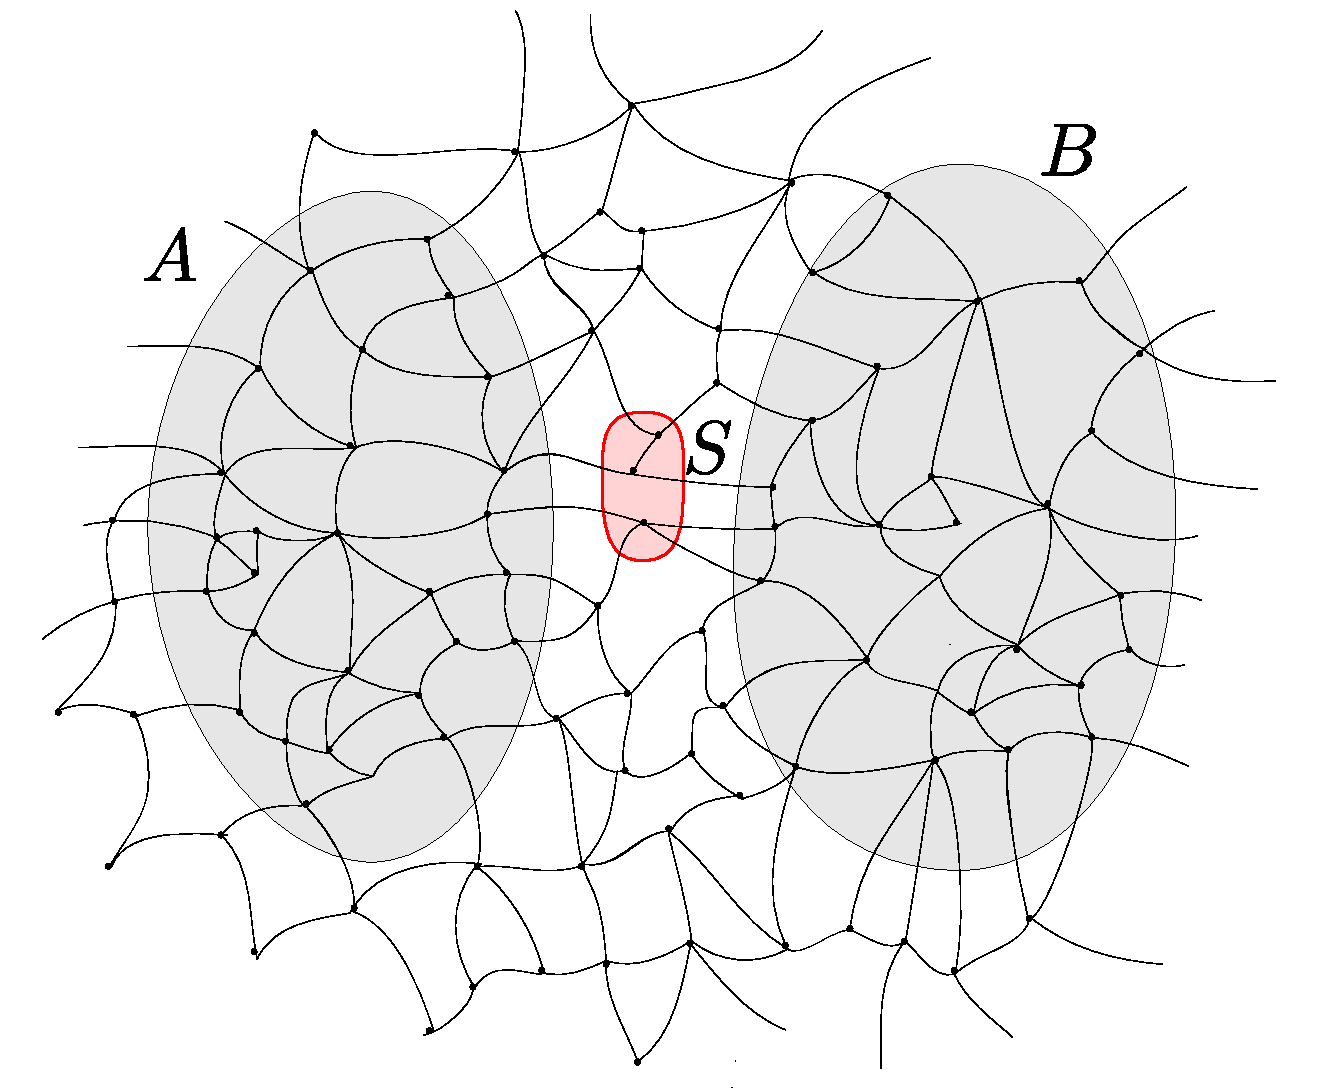
\includegraphics[scale=0.35,page=1]{pics}
 	\caption{The sets $A$ and $B$ are $2$-separated by $S$.
 	}
 	\label{fig:sep}
 \end{figure}
We remark that taking $r=\infty$ in $r$-separation yields the familiar notion of separation in graph theory,
and on the other hand, characterizes \emph{forking independence} in superflat graphs~\cite{ivanov}. Therefore,
$r$-separation can be thought of as a local analogue of forking independence, for nowhere dense graph classes.

A key lemma concerning $r$-separation (cf.~\cref{cor:bound}) states that if $A$
and $B$ are $r$-separated by a set $S$ of size $s$,
then for any fixed formula $\phi(\bar x,\bar y)$,
the set  $\{\{\tup b\ \in B^{|\bar x|} : \strA\models\phi(\tup a,\tup b)\} : \tup a\in A^{|\bar y|}\}$ has cardinality bounded by a constant depending on $s$ and $\phi$ only (and not on $G,A,$ and $B$). This elementary result combines  Gaifman's locality property and a Feferman-Vaught lemma. This, in combination with the polynomial bounds 
for uniform quasi-wideness (\cref{thm:new-uqw}, and its extension to tuples~\cref{thm:uqw-tuples}), as well as the previous results on neighborhood complexity~\cite{eickmeyer2016neighborhood,DrangeDFKLPPRVS16} are the main ingredients of our main result,~\cref{thm:vc-density}.

%
% \paragraph{Stability.}
%
%
% The second topic of study is the
% connection between nowhere denseness and stability theory.
% Fix
% % Let $\cal C$ be a class of structures over
%  a relational vocabulary $\Sigma$. Let
% $\phi(\tup{x},\tup{y})$ be a $\Sigma$-formula with the free variables
% partitioned into two groups $\tup{x}, \tup{y}$. A \emph{$\phi$-ladder}
% of length $n$ in a $\Sigma$-structure $\str A$ is a sequence $\tup{a}_1,\ldots, \tup{a}_{n},
% \tup{b}_1,\ldots, \tup{b}_{n}$ of tuples of elements of $\str A$
% such that for all $1\leq i,j\le n$,
% \[\strA\models\phi(\tup{a}_i,\tup{b}_j)\Longleftrightarrow i\leq j. \]
% The least  $n$ for which
% there is no $\phi$-ladder of length $n$ is
% the \emph{ladder index}
% of $\phi(\tup{x},\tup{y})$ in $\str A$ (which may depend on the way we split the
% variables). A class of graphs $\CCC$ is \emph{stable} if
% the ladder index of every first order formula $\phi(\tup{x},\tup{y})$ over
% graphs from $\CCC$ is bounded by a constant depending only on $\phi$
% and~$\CCC$.
%
% Podewski and Ziegler~\cite{podewski1978stable}
% consider \emph{superflat graphs}, a notion corresponding to uniform quasi-wideness in the
% infinite. They show that flat graphs are stable using an
% infinite Ramsey argument and compactness. Based on the
% results of Podewski and Ziegler,
% Adler and Adler~\cite{adler2014interpreting}
% proved that every nowhere dense class is stable, in fact, they
% proved that for a subgraph-closed class $\CCC$, the notions of
% nowhere denseness and stability coincide.
% However, their inherently non-constructive approach cannot give explicit upper bounds on parameters governing the stability of $\CCC$, for instance, the ladder indices.
%
% Based on the approach of Podewski and Ziegler~\cite{podewski1978stable}, we give a combinatorial
% proof that every first order formula has finite ladder index on every
% nowhere dense class, which does not involve infinite combinatorics and model theory.
% In particular, instead of compactness we use Gaifman's Locality Theorem for
% first order logic~\cite{gaifman1982local}. The following theorem summarizes our~result.
%
% \begin{theorem}\label{thm:new-stable}
%   There are computable functions $f\colon \N^3\to\N$ and $g\colon\N\to\N$ with the following property.
% Suppose $\phi(\bar x,\bar y)$ is a formula of quantifier rank $q$ and with $d$ free variables,
% and $G$ is a graph such that $K_t\not\minor_{g(q)} G$. Then the ladder index of $\phi(\bar x,\bar y)$ in $G$ is at most $f(q,d,t)$.
% \end{theorem}
%
% Note that in particular, \cref{thm:new-stable} implies that every nowhere dense graph is stable, which was the main conclusion of Adler and Adler~\cite{adler2014interpreting}.
%
% We remark that the above connections between nowhere denseness and notions from model theory have recently found algorithmic applications.
% Both uniform quasi-wideness and stability techniques are key tools used in the study of the complexity of the {\sc Distance-$r$ Dominating Set} problem on nowhere dense graph classes,
% and in particular in the design of polynomial kernelization procedures for this problem~\cite{DawarK09,drange2016kernelization,eickmeyer2016neighborhood,siebertz2016polynomial}.


\paragraph{Organization.} In \cref{sec:uqw} we recall standard concepts from the theory of sparse graphs and prove \cref{thm:new-uqw}, improving greatly the previously the previous bounds.
In~\cref{sec:uqw-tuples} we formulate and prove the  generalization to tuples,~\cref{thm:uqw-tuples}. This result is new in the context of nowhere dense graph classes, and is an important tool for the further results.
In \cref{sec:gaifman} we discuss Gaifman locality for first order logic and derive an elementary variant  concerning local separators.
 In \cref{sec:types} we prove our main result, \cref{thm:vc-density}, and of the corresponding lower bounds, given by \cref{thm:vc-density-lower-bound}.
Finally, in \cref{sec:stable} we provide an effective proof of the result of Adler and Adler, \cref{thm:new-stable}.

%\end{change}

%\pagebreak


% Finally, we observe that an argument of Bousquet and
% Thomasse\'e~\cite{BousquetT15} can be slightly modified to prove that
% the VC-dimension of the $r$th power $G^r$ of a graph $G$
% with $K_t\not\minor_r G$ is bounded by $t-1$.
% Boundedness of VC-dimension is a weaker condition than the stability of a class, however it is sufficient in many contexts.
% Therefore, we consider investigating explicit bounds on the VC-dimension potentially useful for future research.
%
% \begin{theorem}\label{thm:new-vc}
% Let $G$ be a graph such that $K_t\not\minor_r G$. Then the
% VC-dimension of $G^r$, the $r$th power of the graph~$G$, is bounded by $t-1$.
% \end{theorem}

%\paragraph{Organization.} We give background from graph theory in \cref{sec:uqw}, where we also
%prove \cref{thm:new-uqw}. 
%We provide background 
%on logic and prove \cref{thm:new-stable} in \cref{sec:stable}. 






\section{Uniform quasi-wideness}\label{sec:uqw}

The $k$-order property of a formula is strongly related
to its branching index. The largest $k$ such that 
$\psi$ has the $k$-order property over $G$ is
also called the \emph{ladder-index} of $\psi$ over $G$. 

If $\tau$ is a word over an alphabet $\Sigma$ and
$a\in \Sigma$, then $\tau\cdot a$ denotes the concatenation of~$\tau$
and $a$.  The \emph{branching index} of a formula $\psi(\tup{x},\tup{y}$
over a graph $G$ is the largest number
$\ell$ such that there are tuples of elements
$\tup{u}_{\sigma_1},\ldots, \tup{u}_{\sigma_{2^\ell}}\in V(G)$, indexed by the
words over the alphabet $\{0,1\}$ of length exactly $\ell$, and
tuples of elements $\tup{v}_{\tau_1},\ldots, \tup{v}_{\tau_{2^\ell-1}}$, indexed by the
words over $\{0,1\}$ of length strictly smaller than $\ell$, such that
if $\tau_j\cdot a$ is a (not necessarily proper) prefix of~$\sigma_i$, then
$G\models \psi(\tup{u}_{\sigma_i},\tup{v}_{\tau_j})$ if, and only if, $a=1$. The tuples
$\tup{u}_{\sigma_1},\ldots, \tup{u}_{\sigma_{2^\ell}}\in V(G)$ are called the 
\emph{leaves} of the tree, the tuples $\tup{v}_{\tau_1},\ldots, \tup{v}_{\tau_{2^\ell-1}}$
are its \emph{inner nodes}. Intuitively, a leaf $\tup{u}$ is connected to its 
predecessors~$\tup{v}$ such
that $\tup{u}$ is a \emph{right successor} of $\tup{v}$ and not to its predecessors such that 
it is a \emph{left
successor}. 
     

\begin{lemma}[\cite{hodges1993model}, Lemma 6.7.9, p.\
  313]\label{lem:branching}
  Let $\psi(\tup{x},\tup{y})$ be a formula and let $G$ be a graph. 
  If $\psi$ has branching index~$k$ over $G$, 
  then~$\psi$ has ladder index smaller than $2^{k+1}$ over $G$. 
  If $\psi$ has  has
  ladder index $k$ over $G$, then $\psi$ has branching index smaller than
  $2^{k+2}-2$ over $G$.
 \end{lemma}

In the proof of~\cref{thm:malshelah} we construct a type tree, in which
elements are iteratively classified according to their types. The depth of 
the type tree is directly related to the branching index of the formula. 
Our first theorem shows that we can avoid the exponential dependency 
between branching index and ladder index if we consider formulas $\psi(x,y)$
with exactly two free variables. 


Let $\psi(x,y)$ be a formula with $2$ free variables and let $(v_1,\ldots, v_n)$
be a sequence of vertices of $G$. The \emph{type tree}
of $\psi$ over $(v_1,\ldots,v_n)$ is constructed as 
follows. We make $v_1$ the root of the tree. Assume that $v_1,\ldots, v_i$
have been inserted to the tree. We follow a root-leaf path to find the
position for the next vertex $v_{i+1}$. If $G\models\psi(v_j,v_{i+1})$, we
go the right branch of the tree, otherwise we go to the left branch of 
the tree. 


\begin{theorem}
Let $\phi(x,y)$ be a formula with $2$ free variables and let
$(v_1,\ldots, v_n)$ be a sequence of elements of $G$. Then the 
largest complete binary subtree that is found as a topological minor 
of the type tree of $\psi$ over
$(v_1,\ldots, v_n)$ has depth at most twice the ladder
index of $\psi$. 
\end{theorem}
\begin{proof}
Consider the alternating path in the tree. 
\end{proof}

The following is implicit in~\cite{malliaris2014regularity}. 

\begin{lemma}[reference?]\label{lem:depth}
If a tree with $n$ vertices does not contain a complete binary 
tree of depth $k$ as a topological minor, then it has depth at most 
$x$. 
\end{lemma}

\begin{lemma}\label{lem:minor-to-tree}
Let $\phi(x,y)$ be a formula with $2$ free variables and let
$(v_1,\ldots, v_n)$ be a sequence of elements of $G$. Let $H$
be the topological minor model of a complete binary subtree in the
type tree of $\psi$ over $(v_1,\ldots, v_n)$. Denote the 
principal vertices of $H$ by $(w_1,\ldots, w_m)$. Then the type
tree of $\psi$ over $(w_1,\ldots, w_m)$ is a complete binary
tree. 
\end{lemma}

For the proof of our theorem we will use the formula 
$\dist_G(x,y)\leq 2$, for which we can give an explicit 
bound on the depth of the largest binary subtree.

\begin{theorem}
Let $\CCC$ be a nowhere dense class of graphs. Let 
$(v_1,\ldots, v_n)$ be the enumeration of an independent set 
in $G$. Assume that $K_t\not\minor_2G$. 
Then the largest complete binary subtree that is found as a topological minor 
of the type tree of $\psi$ over
$(v_1,\ldots, v_n)$ has depth at most $2(t-1)$. 
\end{theorem}
\begin{proof}
According to \cref{lem:minor-to-tree} we may assume that we find
the largest complete binary tree as a subgraph. We consider the
vertices $a_1,b_1,\ldots, a_k,b_k$ of the alternating path in the
type tree. Because $(v_1,\ldots, v_n)$ is independent in $G$, 
none of these vertices is adjacent and all of the vertices on the
paths of length $2$ which cause the creation of edges in the type
tree are distinct from $a_1,\ldots, b_k$. 

\begin{claim}
Every vertex $a_i$ is connected to every $b_j$, $j\geq i$,
via a vertex $z_{ij}$ which is not connected to any~$b_\ell$, $\ell\neq j$. 
\end{claim}

\noindent\textit{Proof.} Because $b_j$, $j\geq i$, is right of $a_i$, there is 
an element $z_{ij}$ connected to $a_i$ and $b_j$. If $z_{ij}$ was 
connected to $b_\ell$, $\ell\neq j$, then $b_\ell$ would be adjacent 
to $b_j$ in the type tree, which it is not. \hfill$\lrcorner$

\bigskip
We now contract $b_j$ and all $z_{ij}$ as well as $a_j$ to a single 
vertex for all $1\leq j\leq k$, $1\leq i\leq j$. We obtain a complete
graph $K_k$ as a depth-$2$ minor. 
\end{proof}

Note that the above proof does not give a proof that the ladder
index of the distance-$2$ formula is at most $2(t-1)$. In the type
tree we have the stronger statement that the vertices $b_i$
are not connected by a path of length $2$. 
We make no statement about the connections
of these elements in the ladder. 

\begin{theorem}
The function $N$ in the definition of uniform quasi-wideness
is small.
\end{theorem}
\begin{proof}
Assume $K_t\not\minor_2G$, in particular, $G$ excludes $K_t$
as a subgraph. We take a large independent subset $A'$ of $A$ and
enumerate it as $(a_1,\ldots, a_m)$. We build the type
tree, which has depth at least $x$ according to \cref{lem:depth}. 
We consider the longest branch of the type tree. On this branch, 
we take a set $X$ of maximum length such that every vertex has 
all its successors on the same side. This set has size at least
half the length of the branch. 

Either, $X$ is a set with all its successors on the left, then $X$ 
is a $2$-independent set and we are done with this step and
continue with $X$. Otherwise, all vertices of $X$ are at distance
$2$. Let $m=X$ and assume that $m$ is larger than $n_0$ to
be defined for neighbourhood complexity.
We claim that we find an element which is connected to at least $m^{1/3}$
of the vertices of $X$. Otherwise, every vertex
can create only $m^{2/3}$ connections, however, we need
to create $m^2$ connections. Hence, we need $m^{4/3}$ vertices
to create all connections. We have neighbourhood complexity
$m^{1+\epsilon}$ though, a contradiction. 

We delete the element of degree $m^{1/3}$ 
and continue with the subsequence
induced by its neighbours. This can happen at most 
$t(2)$ times, as we are constructing a complete minor at 
depth $2$ here. 
\end{proof}


\section{Gaifman locality}\label{sec:gaifman}
In this section, we extract from Gaifman's Locality Theorem~\cite{gaifman1982local} a technical lemma
(\cref{pro:crossing} below), which will be used later in two different settings: in the proofs of \cref{thm:vc-density} and of \cref{thm:uqw-stable}.



If $X,Y,S\subset V(G)$ are sets of vertices of a graph $G$ 
and $r\in \N$, then we say that $X$ and $Y$ are  \emph{$r$-separated}
by $S$  (in $G$) if every path between a vertex in $X$ and a vertex in 
$Y$ of length at most~$r$ contains a vertex from $S$. If $G$ is a graph, $B\subset V(G)$ is a set of vertices,
and $u,v\in V(G)^d$ are two tuples of vertices, then we say that 
$u$ and $v$ have \emph{the same quantifier rank $q$ type} over $B$
if $u$ and $v$ satisfy exactly the same formulas of quantifier rank $q$ with parameters from $B$.
Precisely,
for every $k\in \N$, every tuple $u\in B^{k}$ of $k$ elements of $B$, and every formula $\phi$ of quantifier rank $q$ and with $d+k$ free variables, we have that $\phi(u,w)$ holds if and only if $\phi(v,w)$ holds.




In this section we prove the following technical lemma, which
may be considered folklore. %(cf. Fig~\ref{fig:gaifman} for a graphical illustration). 


\begin{lemma}\label{pro:crossing}	
	% Let $\phi$ be a formula with
	%  quantifier rank $q$ and
	%    free variables $X$
	%  partitioned as $X=Y\cup Z$.
For
every graph $G$, set of vertices $S\subset V(G)$, integers $q,d\in\N$, 
there is a  function mapping tuples  $v\in V(G)^d$
	to \emph{$(q,S)$-local types},
so that the following conditions 
hold.
	 \begin{enumerate}[(1)]
	 	\item\label{c:number} The  set of  $(q,S)$-local types  of all tuples $v\in V(G)^d$  is finite and has size bounded by 
    $T(q,d,|S|)$, for some computable function $T\from \N\times \N\times\N\to \N$ which is non-decreasing in all of its arguments.

	
		
    % \item The $\phi$-type of $v\in V(G)^X$ only depends on the pair $(H,v)$, where $H$ is the subgraph induced by the vertices in $G$
    %     which are within distance at most  $r(q)$  from some vertex in the range of $v$, for some computable function $r(\cdot)$.

		
	 	\item\label{c:confusing}
		 % 	    Let $\phi$ be a formula with
		 % 	   	 quantifier rank $q$,
		 % parameters from $K\subset V(G)$, and free variables $Y$.
		 	  There is a number 
		 $r\in\N$ computable from $q$ with the following property. 
		 If $A,B\subset V(G)$ are 
 $r$-separated by $S$,
then any two tuples $u,v\in A^d$
		 of the same $(q,S)$-local type
have
		 the same  quantifier rank $q$ type
		 over $B$.
		 	%
	%
	%   if $u,v\in V(G)^Y,w\in V(G)^Z$ satisfy:
	%   \begin{itemize}
	% \item  $u$ and $w$ are $r$-independent in $G-S$,
	% \item  $v$ and $w$ are $r$-independent in $G-S$, and
	%   	\item $u$ and $v$ have the same $(q,S,Y)$-types,
	%   \end{itemize}
	%   then
% \[G,u\oplus w\models \phi\iff G,v\oplus w\models \phi.\]
	 \end{enumerate}
\end{lemma}

\begin{comment}
\begin{figure}[h!]
	\centering
		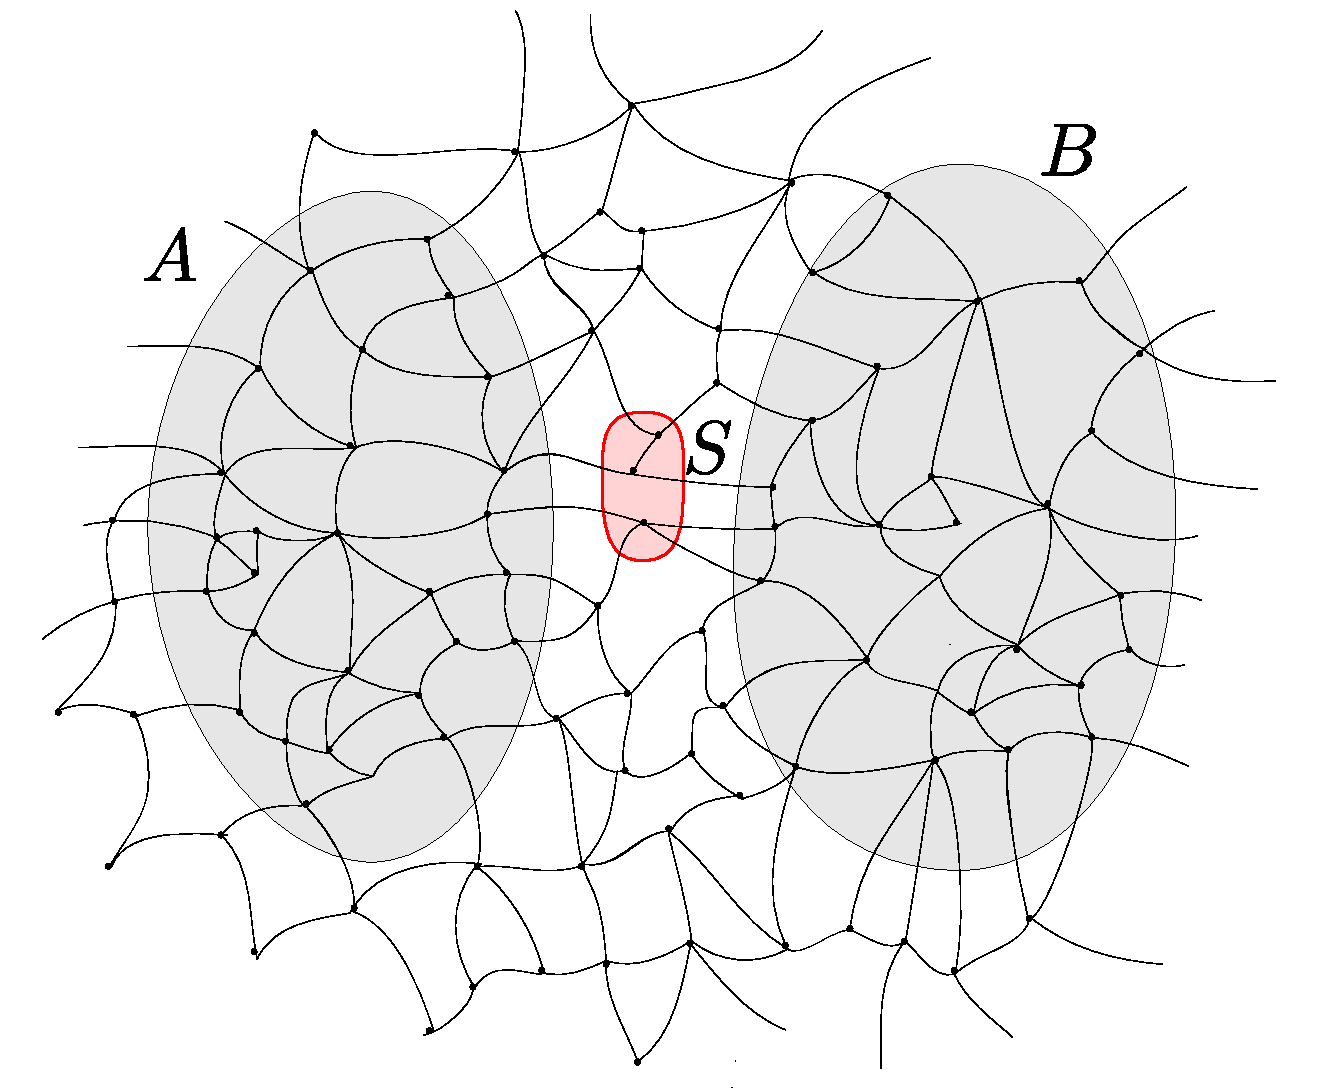
\includegraphics[scale=0.3,page=1]{pics}
	\caption{The sets $A$ and $B$ are $r$-separated by $S$
	(here $r=3$), and the tuples $u,v$ of elements of $A$ are assumed to have  
	the same \emph{$(q,S)$-local type}, where $q\sim \log r$. This implies that 
	for every first-order formula $\phi(\bar x,\bar y)$ of quantifier rank
	$q$
	(where $|\bar x|=|u|=|v|$)
	and every tuple $w$ of $|\bar y|$ elements of $B$,	
	  $\phi(u,w)$ holds in $G$ iff 
	 $\phi(v,w)$ holds in $G$.
	}
	\label{fig:gaifman}
\end{figure}
\end{comment}

The rest of Section~\ref{sec:gaifman} is devoted to the proof of~\cref{pro:crossing}.
We start by introducing some notation which will be used in this proof only.

We consider only finite sets of variables, and any mathematical object can be considered a variable 
(formally, whenever we want to treat an object $a$ as a variable, we introduce a variable~$x_a$, where~$x$ is a fixed special symbol).
If $\phi$ is a formula then it has a specified set of free variables.
By abuse of language, if $X$ is a set of variables and $\phi$
is a formula, when we say that $\phi$ \emph{has free variables}~$X$
we allow the set of free variables of $\phi$ to be a subset of $X$.

If $X$ is a finite set and $V$ is a set, then $V^X$ denotes the set of functions from $X$ to $V$, and an element $v\in V^X$ will be sometimes called a \emph{tuple} 
or, in the case $X$ is a set of variables, a \emph{valuation} of $X$.
For two tuples
$v\in V^Y$ and $w\in  W^Z$, where $Y$ and $Z$ are disjoint, by
$v\oplus w$ we denote the set-theoretic union of the functions $v,w$,
which is a tuple $v\oplus w\in (V\cup W)^{Y\cup Z}$.
The image of a valuation $v$ is denoted by $\im(v)$.


% If $V=V(G)$ for some graph $G$, then we can treat valuations of~$X$ as tuples of length $|X|$ consisting of vertices of $G$, ordered in the same way according to any fixed enumeration of $X$.
% Then we may say that a set of valuations is mutually $r$-independent in~$G$, or in $G-S$ for some $S\subseteq V(G)$, meaning the notion discussed in the previous section.


Fix a formula $\phi$ with free variables $X$.
Given a valuation $v\in V(G)^X$, we write $G,v\models \phi$ to denote that $\phi$ is satisfied 
in the graph $G$ with valuation $v$, which is defined as usual in logic, by induction on the structure of $\phi$.




It remains to prove~\cref{pro:crossing}. 
First we recall some notions from logic, namely quantifier ranks, Gaifman's Locality Theorem, and some simple manipulations on formulas.

 Fix a finite set of  colors $C$.
By a \emph{colored graph} we mean a graph  in which 
every vertex is assigned zero or more colors from $C$. We view a colored graph as a relational structure as usual, by treating each color as a unary predicate. 

The \emph{quantifier rank} of a formula $\phi$ is the maximal number of nested quantifiers in $\phi$.
For $i=1,2$, let $G_i$
be a colored graph and $v_i:X\to V(G_i)$ be a valuation
from a common set of variables $X$.
We say that $(G_1, v_1)$ and $(G_2,v_2)$
have the same \emph{quantifier rank $q$ type} %\marginpar{also called $q$-equivalent and denoted $(G_1,\bar v_1)\equiv_q (G_2, \bar v_2)$}
if for every formula $\phi$ with  free variables $X$ and of quantifier rank $q$,
 $$G_1,v_1\models \phi\qquad\iff \qquad G_2,v_2\models \phi.$$
If $G$ is a graph colored with colors from $C$ and 
 $v\from X\to V(G)$ is a valuation, 
then the equivalence class of $(G, v)$ under the above equivalence relation is called the \emph{quantifier rank $q$ type} of $(G,v)$, and  the set of \emph{quantifier rank $q$ types with  free variables $X$}
is the set of all equivalence classes, denoted
$\mathrm{Tp}^{q,C}_X$.

 If $G$ is a colored graph, $r\in\N$ is an integer, and $v$ is a valuation of a set of variables in $G$, then  $N^G_r[v]$ denotes the pair $(H,v)$, where $H$ is the colored subgraph of $G$
induced by the set of all vertices which are in distance at most $r$
from some vertex in the image of $v$.
If $r$ is an integer, then the \emph{$(r,q)$-local type} of $(G,v)$ is 
the quantifier rank $q$ type of $N^G_r[v]$. The $q$-\emph{local type} of $(G,v)$ is the $(r,q)$-local type, where $r$   is the value described in the second item of the following proposition,  summarizing several well-known properties of types and local types.


\begin{proposition}\label{pro:gaifman}
	Fix a positive integer $q$, a finite set of colors $C$, and a set of variables $X$. Let~$G$ be any $C$-colored graph. Then the following conditions hold:
 \begin{enumerate}[(1)]
 	\item \emph{(Computability of types)} The set of types $\mathrm{Tp}^{q,C}_X$ is finite and computable from $C$, $X$, and $q$.

	\item \emph{(Locality of first order logic)} There is an integer $r$ computable from $q$ such that for every formula $\phi$ in the signature of $C$-colored graphs  
	of quantifier rank $q$ and with free variables~$X$,	
  if $(G,v_1)$ and $(G,v_2)$ have the same $(r,q)$-local types,
	then
	 $$G,v_1\models \phi\qquad\iff \qquad G,v_2\models \phi.$$
   % We call $r$ the \emph{locality radius} for quantifier rank $q$, and fix this number in what follows.

%    \item \emph{(Monotonicity)} If $Y\subset X$ and $v \from X\to V(G)$
%    is a valuation, then the $(q,r)$-local type of $(G,v)$
% determines   the $(q,r)$-local type $(G,v|_Y)$ of the restriction of $v$ to $Y$.


	 \item \emph{(Independence)} Suppose $X$ is partitioned into $Y\cup Z$, 
	 and that $u_1,u_2\from Y\to V(G)$ and $v_1,v_2\from Z\to V(G)$ are valuations
   such that  $u_1$ and $v_1$, as well as $u_2$ and $v_2$,
   are $2r$-independent in $G$, for some $r$.
   Moreover, suppose that the $(r,q)$-local types of $(G,\im(u_1))$ and $(G,\im(u_2))$ are equal,
   and that the $(r,q)$-local types of $(G,\im(v_1))$ and $(G,\im(v_2))$ are equal.
   Then the $(r,q)$-local types of $(G,u_1\oplus v_1)$ and $(G,u_2\oplus v_2)$ are equal.
 \end{enumerate}
\end{proposition}


\begin{proof}%[of~\cref{pro:gaifman}]

\emph{Computability of types} is standard~(see e.g. Lemma 3.13 in~\cite{libkin}).
% and  yields the first condition in~\cref{pro:gaifman}.
% \begin{lemma}\label{lem:q-types}
%   Fix a set of colors $C$, a rank $q$ and a set of variables $X$.
%   Then the set $\mathrm{Tp}^{q,C}_X$ of quantifier rank $q$ types with free variables $X$ is finite and computable.
% \end{lemma}

\emph{Locality of first order logic} is an
immediate consequence of Gaifman's Locality Theorem
(the Main Theorem~in~\cite{gaifman1982local}),
where it is shown that one can take $r=7^q$.
It is also known (cf. Exercise~4.10 in \cite{libkin}) that it suffices to take $r=2^q$; this bound is tight.


% We say that a formula $\phi(\bar x)$ with $d=|\bar x|$ free variables is \emph{$q$-local} if for every colored graph $G$ and every $\bar a_1,\bar a_2\in V(G^d)$, if  $N^G_r(\bar a_1)$ and  $N^G_r(\bar a_2)$
% are isomorphic, then $G,\bar a_1\models \phi(\bar x)$ if and only if $G,\bar a_2\models \phi(\bar x)$.
%
% \begin{lemma}\label{lem:gaifman}
%   Let $\phi$ be a  formula
%   of quantifier rank $q$
%   in the signature of colored graphs, with free variables $X$.
%   Suppose $v_1,v_2$ are valuations of $X$ in $G$ such that $N^G_r[v_1]$ and $N^G_r[v_2]$ have the same quantifier rank $q$ type, where $r=7^q$. Then
%  $$G,v_1\models \phi\qquad\iff \qquad G,v_2\models \phi.$$
% \end{lemma}

% We also use the following well-known fact about the compositionality of types
% under taking disjoint unions. The proof is a standard application of Ehrenfeucht-Fraisse games, so we only give a sketch.
For \emph{Independence}, write $G\oplus H$ for the disjoint union of colored graphs $G,H$. 
We use the following claim, whose proof is a standard application of Ehrenfeucht-Fraisse games.


		\begin{claim}\label{lem:type-union}
			For $i=1,2$, let $G_i,H_i$ be colored graphs,
			and $v_i\from Y\to V(G_i)$ and $w_i\from Z\to V(H_i)$ be valuations.
			Suppose that $(G_1,v_1)$ and $(G_2,v_2)$ 
			have the same quantifier rank $q$ type,
			and $(H_1,w_1)$ and $(H_2,w_2)$ 
			have the same quantifier rank $q$ type.
			Then the quantifier rank $q$ type of the disjoint union 
			$(G_1\oplus H_1,v_1\oplus w_1)$ is equal to the one of $(G_2\oplus H_2,v_2\oplus w_2)$. \end{claim}
\begin{clproof}[Sketch]
	The proof proceeds by applying the well-known characterization 
	of quantifier rank $q$  types using Ehrenfeucht-Fraisse games (see e.g. Theorem 3.9 in~\cite{libkin}). By assumption, duplicator has a winning strategy $\gamma$ in the $q$-round game on $(G_1,v_1)$ and $(G_2,v_2)$, and a winning strategy $\eta$ in the $q$-round game on $(H_1,w_1)$ and $(H_2,w_2)$. The strategies $\gamma$ and $\eta$ can be combined into a winning strategy on $(G_1\oplus H_1,v_1\oplus w_1)$  and $(G_2\oplus H_2,v_2\oplus w_2)$.
\end{clproof}
The \emph{Independence} property is now almost immediate. Since $u_1$ and $v_1$ are $2r$-independent in $G$, the subgraph of $G$ induced by the $r$-neighborhood of $\im(u_1\oplus v_1)$ is isomorphic to the disjoint union of the subgraphs of $G$ induced by the $r$-neighborhoods of $\im(u_1)$ and $\im(v_1)$. The same holds also for the $r$-neighborhoods of $\im(u_2\oplus v_2)$, 
$\im(u_2)$, and $\im(v_2)$. It now suffices to apply \cref{lem:type-union} and use the assumed equality of $(r,q)$-local types.
\end{proof}

We now prove \cref{pro:crossing}. Until the end of the proof, fix a graph $G$ and a set of vertices $S\subset V(G)$.
We now introduce some notation allowing to translate a  formula~$\phi$ talking about  $G$ into an equivalent formula $\phi'$ talking 
about a suitably colored  graph $G$ with the set of vertices $S$ removed.
Precisely, define the structure $G^{S}$
as the graph $G-S$ colored with colors $\set{C_s\colon s\in S}$ as follows.
For each $s\in S$, a vertex $v\in V(G)-S$
is colored with color $C_s$ in $G^S$ if and only if $v$ is a neighbor of $s$
in~$G$.

Fix a formula $\phi$ with free variables $X$.
If $G$ is a (colored) graph, $S\subset V(G)$ is a set of vertices, and $Y$ is a set of variables disjoint from $V(G)$, then 
a \emph{pre-valuation} in $Y\cup S$ is a 
function $\alpha\colon X\to Y\cup S$.
If $v\from Y\to V(G)$ is a valuation and $\alpha$ is as above,
then by $\alpha\cdot v$ we denote the valuation of $X$ in $V(G)$
which maps $x\in X$ to $\alpha(x) $ if $\alpha(x)\in S$
and to $v(\alpha(x))$ if $\alpha(x)\in Y$.
 The  pair $(\phi,\alpha)$  can be treated as a
syntactic object denoted  $\phi^{\alpha}$,
 whose semantics is defined so that for a valuation $v\from Y\to V(G)$, 
$$G,v\models \phi^{\alpha}\qquad\iff \qquad G,\alpha\cdot v\models \phi.$$
Intuitively $\phi^\alpha$ is the formula $\phi$ with variable $x$ substituted by $\alpha(x)$,
which can be either a variable in $Y$ or a vertex in $S$, treated as a constant.


\begin{lemma}\label{lem:remove-s}Let $G,S$ be as above.	
For every formula $\phi$ with free variables $X$ and every pre-valuation $\alpha\from X\to Y\cup S$
there is a formula $\phi'$ with free variables $Y$
of the same quantifier rank as $\phi$ and over the signature of $G^S$
 such that for every valuation $v$ of $Y$ in $G-S$, we have
$$G,v\models\phi^{\alpha}\qquad\iff\qquad G^S,v\models\phi'.$$
\end{lemma}
\begin{proof}
The proof proceeds by induction on the structure of the formula $\phi$. 

If $\phi$ is an atomic formula $E(x,x')$ or $x=x'$, then the formula $\phi'$ is constructed by case analysis. If $\alpha(x),\alpha(x')\in Y$ then $\phi'$
is obtained from $\phi$ by substituting the variables $x,x'$ with variables from $Y$ according to~$\alpha$. If  $\alpha(x),\alpha(x')\in S$ then $\phi'$ is the truth value $\bot$ or $\top$ of 
the formula $\phi$ in the graph $G$ under the valuation which maps $x$ to $\alpha(x)$ and $x'$ to $\alpha(x')$. Finally, suppose that $\alpha(x)=y\in Y$ and $\alpha(x')=s\in S$. If $\phi$ is $E(x,x')$ then $\phi'$ is the formula $C_{s}(y)$, and if $\phi$ is $x=x'$ then $\phi'$ is the formula $\bot$.
 
 

%
% then, depending on whether $\alpha(x),\alpha(x')$ belong to $Y$ or to $S$, we consider  the appropriate case in the list below, where $y,y'$ range over $Y$ and $s,t$ range over $S$:
% \begin{enumerate}
% 	$E(y,y')\mapsto E(y,y')$
%
% 	\item If $\alpha(x)=y$ and $\alpha(x')=y'$ then $\phi'$ is $E(y,y')$.
% 	\item If $\alpha(x)=y$ and $\alpha(x')=s$ then $\phi'$ is $C_s(y)$.
% 	\item If $\alpha(x)=s$ and $\alpha(x')=y'$ then $\phi'$ is $C_s(x')$.
% 	\item If $\alpha(x)=s$ and $\alpha(x')=t$ then $\phi'$ is $\top$ if $s$ and $t$ are adjacent in $G$ and $\bot$ otherwise.
% \end{enumerate}
% We proceed similarly when $\phi$ is an atomic formula $x=x'$:
% \begin{enumerate}
% 	\item If $\alpha(x)=y$ and $\alpha(x')=y'$ then $\phi'$ is $y=y'$.
% 	\item If $\alpha(x)=y$ and $\alpha(x')=s$ then $\phi'$ is $\bot$.
% 	\item If $\alpha(x)=s$ and $\alpha(x')=y'$ then $\phi'$ is $\bot$.
% 	\item If $\alpha(x)=s$ and $\alpha(x')=t$ then $\phi'$ is $\top$ if $s=t$ are adjacent in $G$ and $\bot$ otherwise.
% \end{enumerate}





For the inductive step, we consider two cases.
If $\phi$ is a boolean combination of formulas $\phi_1,\ldots,\phi_k$, then 
apply the inductive assumption to each formula $\phi_i$,
yielding formulas $\phi_1',\ldots,\phi_k'$. Then let $\phi'$ be the analogous boolean combination of the formulas $\phi_1',\ldots,\phi_k'$.

Finally, suppose that $\phi$ is of the form $\exists x.\psi$, where   $Y$ are the free variables of $\phi$ and $x\not \in Y$.
 For $w$ being either the variable $x$ 
or an element $s\in S$, 
let $\psi^w$ be the formula obtained from the inductive assumption applied to the formula $\psi$ 
and pre-valuation $\alpha$ extended to a valuation which maps  $x$ to $w$. 
Then let $\phi'$
be the formula $\exists x.\psi^x \lor \bigvee_{v\in S}\psi^v$.
The case of $\forall$ is dual.

In each case, it follows from the inductive assumption that $\phi'$ 
satisfies the required condition.
\end{proof}



Let $X$ be a set of variables.
For a valuation  $v$ of $X$ in $G$, we introduce the notion of an \emph{$S$-decomposition} of $v$,  
which is the (essentially unique) pair $(\alpha,v^S)$
such that $\alpha\from X\to Y\cup S$ is a pre-valuation
for some set of variables $Y$,
and $v^S\from Y\to (\im(v)-S)$ is a bijective valuation such that 
$\alpha\cdot v^S=v$. The formal definition is as follows.
% Let $\sim$ be the partial equivalence on $X$ defined so that
% $x\sim x'$ if and only if both $x$ and $x'$ are mapped to the same element of $Y$.
% In other words, $\sim$ is the restriction of the kernel of $v$ to $v^{-1}(Y)$.
Let $Y=\set{v^{-1}(\set u)\colon u\in \im(v)-S}$. We treat $Y$ as a set of variables. 
% Note that $Y$ is in bijection with $\rg(v)-S$, but we prefer
% to define $Y$ in a way which is independent of the elements of $G-S$ for technical reasons.
Define the pre-valuation $\alpha\from X\to Y\cup S$
by letting $\alpha(x)$ be $v(x)$ if $v(x)\in S$,
and $v^{-1}(\set u)$ if $v(x)=u$ for some $u\in \im(v)-S$.
Finally, let $v^S$ be the valuation of $Y$ in $G$ which
maps  $v^{-1}(\set u)$ to $u$, for $u\in \im(v)-S$.
It is easy to see that $v=\alpha\cdot v^S$ and $v^S$ is a bijection from $Y$ 
to $\im(v)-S$. We call the pair $(\alpha,v^S)$ the \emph{$S$-decomposition of $v$}.


\begin{definition}\label{def:}
For a number $q$ and valuation $v\from X \to V(G)$, the \emph{$(q,S)$-local type} of $v$ 
is the pair $(\alpha,\tau)$,
where $(\alpha,v^S)$ is the $S$-decomposition of~$v$
and $\tau$ is the $q$-local type of   $(G^S,v^S)$.	
\end{definition}
Note that there are at most  $(s+d)^d$ possible functions $\alpha$, where $s=|S|$ and $d=|X|$. In particular, by the computability of types (cf.~\cref{pro:gaifman}), 
the number of $(q,S)$-local types of valuations from~$X$
in arbitrary graphs is bounded by 
a number computable from $s,d$, and $q$.
Therefore, condition~\eqref{c:number} of~\cref{pro:crossing} is satisfied. We are left with verifying condition~\eqref{c:confusing}. For this, we prove another lemma.





\begin{lemma}\label{lem:coloring}
	Let $\phi$ be a formula with
free variables $X$ and of quantifier rank $q$.
	Suppose that~$u$ and~$v$ are two valuations of $X$  in $G$ with the same $(q,S)$-local types.
	Then $$G,u\models \phi\qquad \iff\qquad G,v\models \phi.$$
\end{lemma}
\begin{proof}
Let $(\alpha,\tau)$ be the $(q,S)$-local type of the valuations $u$ and $v$, where $\alpha\from X\to Y\cup S$ for some set of variables $Y$. Let $(\alpha,u^S)$ be the $S$-decomposition of $u$
and let $(\alpha,v^S)$ be the $S$-decomposition of $v$.
	Consider the formulas $\phi^{\alpha}$ and $\phi'$ as described in \cref{lem:remove-s}, both with free variables $Y$.
	In particular, the following equivalences hold:
	\begin{align*}
	G,u\models\phi\iff G,u^S\models\phi^{\alpha}\iff G^S,u^S\models\phi',\\
	G,v\models\phi\iff G,v^S\models\phi^{\alpha}\iff G^S,v^S\models\phi'.
	\end{align*}
		Note that $\phi'$ has the same quantifier rank as  $\phi$, that is, $q$.
		Since $u$ and $ v$ have the same $(q,S)$-local type $\tau$, it follows that $(G^S,u^S)$ and $(G^S,v^S)$ have the same   $q$-local type.
		By the locality of first order logic (cf.~\cref{pro:gaifman}) applied to $G^S$, $\phi'$, $ u^S$, and $v^S$, we infer that $G^S,u^S\models\phi'$ if and only if $G^S,v^S\models\phi'$.
		The lemma follows by combining this with the above equivalences.
\end{proof}

% For a graph $G$, a set of vertices $S\subset V(G)$, a set of variables $X$, and  valuations $u,v$ of $X$ in $G$, we say that $u,v$ are mutually $2r$-independent in $G-S$
% if, when treating $u$ and $v$ as  tuples of length $|X|$,
% the set  $\set{u,v}$ is mutually $2r$-independent in $G-S$.


% \begin{lemma}\label{lem:crossing}	Let $\phi$ be a formula with
% 	 whose set of free variables $X$ is partitioned into  disjoint sets $Y,Z$.
% Let $u$ and $v$ be valuations of $X$ in $G-S$ which, treated as tuples,
% are mutually $2r$-independent in $G-S$, i.e.,  $u(x)$ and $v(x')$ are at distance larger than $2r$ in the subgraph of $G$ induced by $V(G)-S$,
% for $x,x'\in X$.
% Let $u_Y$ and $u_Z$ be the restrictions of $u$ to $Y$ and $Z$ respectively,
% and let $v_Y$ and $v_Z$ be the restrictions of $v$ to $Y$ and $Z$ respectively.
%   Suppose that $u_Y$ and $v_Y$ have the same $q$-local type, and that $u_Z$ and $v_Z$ have the same $q$-local type. Then
%   the valuations $u_Y\oplus v_Z$ and $v_Y\oplus v_Z$
%   of $X$ in $G-S$
%   have the same $q$-local types. In particular,
% $$G,u_Y\oplus v_Z\models \phi\iff G,v_Y\oplus v_Z\models \phi.$$
% \end{lemma}
Finally, we prove~\cref{pro:crossing}.
\begin{proof}[of~\cref{pro:crossing}]
Let $\phi$ be a formula
	of  quantifier rank $q$
   whose free variables $X$ are partitioned into $Y$ and $Z$.
  Let $C$ be the set of colors $\set{C_s:s\in S}$.
  Let $r$ be the number given by the locality of first order logic (cf.~\cref{pro:gaifman}).
  
Let $G$ be a graph $S\subset V(G)$ its subset, and $A,B\subset V(G)$  two sets which are $r$-separated by $S$. Let $u,v\in A^Y$ be two tuples of the same $(q,S)$-local type. We show that $u$ and $v$ have the same quantifier rank $q$-type over $B$. To this end, let $w\in B^Z$ be a tuple of parameters,
and let $\phi$ be a quantifier rank $q$ formula with free variables $ Y\cup Z$.
	

\begin{claim}\label{cl:sametype}
The valuations $u\oplus w$ and $v\oplus w$ have the same 
$(q,S)$-local types.  
\end{claim}
\begin{clproof}
Let $(\alpha,u^S),(\beta,v^S),(\gamma,w^S)$ denote the $S$-decompositions of  $u,v,w$, respectively. 
Clearly, $\im(u)\cap\im(w)\subset A\cap B\subset S$ and $\im(v)\cap \im (w)\subset A\cap B\subset B$.
This implies that the $S$-decompositions of $u\oplus w$
and of  $v\oplus w$ can be computed in a component wise fashion, and are as follows:
\begin{align}
u\oplus w &\colon \quad (\alpha\oplus \gamma,  u^S\oplus w^S)\label{eq:dec1},\\  
v\oplus w &\colon \quad (\beta\oplus \gamma, v^S\oplus w^S)\label{eq:dec2}.
\end{align}
The assumption that $u,v$ have the same $\phi$-type implies the following:

\begin{itemize}
  \item  $\alpha=\beta$.
  In particular, the $S$-decompositions
  \eqref{eq:dec1} and \eqref{eq:dec2}  have the first components equal.
  
    \item The valuations $u^S$ and  $v^S$ have 
  the same $q$-local types.
The fact that $A$ and $B$ are $r$-separated by $S$ implies that $u^S$ and $w^S$
are  $2r$-independent in $G^S$.
  By the independence property of~\cref{pro:gaifman}, the second components of the $S$-decompositions~\eqref{eq:dec1} and~\eqref{eq:dec2}
  have the same $q$-local type. 
\end{itemize}
The two observations above yield the conclusion of the claim.
\end{clproof}
By \cref{cl:sametype} and \cref{lem:coloring} we infer that $u\oplus w\models \phi$ if and only if $v\oplus w\models 
\phi$, proving~\cref{pro:crossing}.
\end{proof}
\section{On the number of types in nowhere dense graph classes}

In this section we prove \Cref{thm:vc-density}, \Cref{thm:vc-density-exp} and \Cref{thm:vc-density-lower-bound}. Recall that for a
formula $\psi(\tup x,y)$, where 
$\tup x$ is an $m$-tuple of variables and $y$ is a single variable, 
\[S_\psi(A,G)=\{\{a\ \in A : G\models\psi(a,\tup v)\} : \tup v\in V(G)^m\}.\]

First, observe that if $A\subseteq B$, then the number of types
over $A$ cannot be larger than the number of types over $B$. 

\begin{lemma}\label{lem:types-over-B}
Let $G$ be a graph and let $A\subseteq B\subseteq V(G)$. Let 
$\psi(\tup x,y)$ be a first-order formula. Then 
$|S_\psi(A,G)|\leq |S_\psi(B,G)|$. 
\end{lemma}

We will first enlarge the set of interest such 
that the connections from outside are well controlled. This approach
was first used in Drange et al.~\cite{drange2016kernelization} for
classes of bounded expansion and extended to nowhere dense
classes in Eickmeyer et al.~\cite{eickmeyer2016neighborhood}. 

Let $G\in \CCC$ be a graph and let $A\subseteq V(G)$ be a subset of vertices. For vertices $v\in A$ and $u\in V(G)\setminus A$, a path $P$ connecting $u$ and $v$ is called {\em{$A$-avoiding}}
if all its vertices apart from~$v$ do not belong to $A$. For a positive integer $r$, the {\em{$r$-projection}} of any $u\in V(G)\setminus A$ on $A$, denoted $M^G_r(u,A)$ is the set of all vertices $v\in A$ that
can be connected to $u$ by an $A$-avoiding path of length at most $r$. The {\em{$r$-projection profile}} of a vertex $u\in V(G)\setminus A$ on $A$ is a function $\rho^G_r[u,A]$ mapping vertices of
$A$ to $\{0,1,\ldots,r,\infty\}$, defined as follows: for every $v\in A$, the value $\rho^G_r[u,A](v)$ is the length of a shortest $A$-avoiding path connecting $u$ and~$v$, and~$\infty$ in case this length
is larger than $r$. We define 
\[\projnum_r(G,A)=|\{M_r^G(u,A)\colon u\in V(G)\setminus A\}|\quad\textrm{and}\quad \projprof_r(G,A)=|\{\rho_r^G[u,A]\colon u\in V(G)\setminus A\}|\]
to be the number of different $r$-projections and $r$-projection profiles realized on $A$, respectively. Clearly, it holds that $\projnum_r(G,A)\leq \projprof_r(G,A)$.

\begin{lemma}[[\cite{drange2016kernelization,eickmeyer2016neighborhood}]\label{lem:closure}
Let $\CCC$ be a class of graphs. 
\begin{enumerate}
\item If $\CCC$ has bounded expansion, then there is a function $\fcl(r)$ and a polynomial-time algorithm that, given $G\in \CCC$, $X\subseteq V(G)$ and $r\in \N$ computes the {\em{$r$-closure}} of $X$, denoted $\cl_r(X)$
with the following properties. 
\begin{itemize}
  \item $X\subseteq \cl_r(X)\subseteq V(G)$;
  \item $|\cl_r(X)|\leq \fcl(r)\cdot |X|$; and
  \item $|M_r^G(u,\cl_r(X))|\leq \fcl(r)$ for each $u\in V(G)\setminus \cl_r(X)$.
\end{itemize}
\item If $\CCC$ is nowhere dense, then there is a function $\fcl(r,\epsilon)$ and a polynomial-time algorithm that, given $G\in \CCC$, $X\subseteq V(G)$, $r\in \N$, and $\epsilon>0$, computes the {\em{$r$-closure}} of $X$, denoted $\cl_r(X)$
with the following properties. 
\begin{itemize}
  \item $X\subseteq \cl_r(X)\subseteq V(G)$;
  \item $|\cl_r(X)|\leq \fcl(r,\epsilon)\cdot |X|^{1+\epsilon}$; and
  \item $|M_r^G(u,\cl_r(X))|\leq \fcl(r,\epsilon)\cdot |X|^{\epsilon}$ for each $u\in V(G)\setminus \cl_r(X)$.
\end{itemize}
\end{enumerate}
\end{lemma}

\begin{lemma}[\cite{drange2016kernelization,eickmeyer2016neighborhood}]\label{lem:projection-complexity}
Let $\CCC$ be a class of graphs. 
\begin{enumerate}
\item If $\CCC$ has bounded expansion, then there is 
  a function $\fproj(r)$ such that for every $r\in \N$, graph $G\in \CCC$, and vertex subset $A\subseteq V(G)$, 
  it holds that $\projprof_r(G,A)\leq \fproj(r)\cdot |A|$.
  \item If $\CCC$ is nowhere dense, then there is 
  a function $\fproj(r,\epsilon)$ such that for every $r\in \N$, 
  $\epsilon>0$, graph $G\in \CCC$, and vertex subset $A\subseteq V(G)$, 
  it holds that $\projprof_r(G,A)\leq \fproj(r,\epsilon)\cdot |A|^{1+\epsilon}$.
\end{enumerate}
\end{lemma}

We now are ready to count the number of types realized by elements
of the same projection class. 

\begin{lemma}\label{lem:num-types-same-class}
Let $\phi(\tup x,y)$ be a first-order formula of locality radius $r$. 
Let $\CCC$ be a class of graphs. 
\begin{enumerate}
\item Assume that $\CCC$ has bounded expansion. Let 
$G\in \CCC$ and $B\subseteq V(G)$. Assume that 
$|M_r^G(u,B)|\leq c$ for some positive integer
$\fcl(r)$. Let $v_1,\ldots, v_t$ be a maximal set
of elements which have different $B$-types and which
have the same $B$-projection. Then $t< (tp_{q,s}+c+1)^{p(r)}$. 

\item Assume that $\CCC$ is nowhere dense. Let 
$G\in \CCC$ and $B\subseteq V(G)$. Let $\epsilon>0$ 
and assume that 
$|M_r^G(u,B)|\leq \fcl(r,\epsilon)\cdot |B|^\epsilon$. 
Let $v_1,\ldots, v_t$ be a maximal set
of elements which have different $B$-types and which
have the same $B$-projection. Then $t< (tp_{q,s}+|B|^\epsilon+1)^{p(r)}$. 
\end{enumerate}
\marginpar{here, nowhere dense suffices and all numbers with $c$}
\end{lemma}
\begin{proof}
Assume $t\geq (tp_{q,s}+c+1)^{p(r)}$. Then by uniform
quasi-wideness, there exists a set $S$ and elements 
$w_1,\ldots, w_m$ which are $2r$-independent in $G-S$. 
Here, $m\geq tp_{q,s}+c+1$. Because $|M_r(u,B)|\leq \fcl(r,\epsilon)\cdot |B|^{\epsilon}$, and no two elements $w,w'$ among
$w_1,\ldots, w_m$ can reach the same element of $B$
in $G-S$, there are at most $\fcl(r,\epsilon)|B|^\epsilon$
elements which reach an element of $B$ in $G-S$. 
Hence, there remain $tp_{q,s}$ elements which have
an empty intersection with $B$ in their $N_r^{G-S}(w)$. 
By \Cref{lem:coloring}, 
the type of the elements depends only on the local $q-S$-type. 
As we have $tp_{q,r}+1$ elements, two of them have the
same type. This is a contradiction with our assumption. 
\end{proof}

Now, it is easy to conclude the main theorem. 

\marginpar{set counter}
\begin{theorem}\label{thm:vc-density}
Let $\CCC$ be a nowhere dense class of graphs, 
let $\epsilon>0$ and let $\psi(\tup x,y)$ be a first-order formula, where 
$\tup x$ is an $m$-tuple of variables and $y$ is a single variable. 
There exists a constant~$c$ such that for every $G\in \CCC$ 
and every
$A\subseteq V(G)$, we have 
\[|S_\psi(A,G)|=|\{\{\tup a\ \in A^m : G\models\psi(\tup a,v)\} : v\in V(G)\}|\leq c\cdot |A|^{1+\epsilon}.\]
\end{theorem}
\begin{proof}
Compute the closure $B$ of $A$ according to \Cref{lem:closure}. 
According to \Cref{lem:types-over-B}, it suffices to bound the
number $|S_\psi(B,G)|$. Now plug the numbers of 
\Cref{lem:closure} and \Cref{lem:projection-complexity} 
into \Cref{lem:num-types-same-class} and conclude. 
\end{proof}

\section{From uniform quasi-wideness to stability}\label{sec:stable}
The main result of this section is Theorem~\ref{thm:uqw-stable},
which states 
that a class of graphs which is uniformly quasi-wide is stable.
In Section~\ref{sec:uqw-tuples} we formulate a consequence of the uniform quasi-wideness which
holds for tuples of vertices. In Section~\ref{sec:uqw-stable} we prove Theorem~\ref{thm:uqw-stable}
using Gaifman's Locality Theorem.


\subsection{Uniform quasi-widness for tuples}\label{sec:uqw-tuples}
Fix a graph $G$, a number $d\in\N$ (the dimension) and a number $r\in \N$ (the radius).
If $S\subset V(G)$ is a set of vertices and $A\subset V(G)^d$ is a set of $d$-tuples of vertices,
then we say that $A$ is $r$-\emph{totally independent} in $G-S$ 
if the set of all vertices $v\in G-S$ which appear on some coordinate of some tuple $\bar a\in A$
is $r$-independent in $G-S$. 


\begin{proposition}\label{prop:uqw-tuples}
	Let $\cal C$ be a uniformly quasi-wide class of graphs and $d\in\N$ a number.
	There is a  function $N^d:\N\times\N\to\N$ and a function $s^d:\N\to\N$
	such that for all $r,m\in\N$ and all subsets $A\subset V(G)^d$
	with $|A|\ge N^d(r,m)$ there  is a set $S\subset V(G)$
	of size $|S|\le s^d(r)$ and a subset $B\subset A$ of size $|B|\ge m$ which is totally $r$-independent in $G-S$.
\end{proposition}
\begin{proof}We fix a uniformly quasi-wide class $\cal C$ and functions $N:\N\times\N\to \N$
	and $s:\N\to\N$ as in the definition of uniform quasi-wideness.
	Let $d\in \N$ be a fixed dimension.
		For a fixed graph $G\in \cal C$  and
	  coordinate $i\in\set{1,\ldots,d}$, let $\pi_i$ denote the projection from $V(G)^d$ onto the $i$th coordinate.

	


\begin{lemma}\label{lem:step1} For any $r,m\in \N$ there is a number $K(r,m)$ such that
	for any given $A\subset V(G)^d$ with $|A|\ge K(r,m)$,
	there is a set $B\subset A$ with $|B|\ge m$ and a set $S\subset V(G)$ with $|S|\le d\cdot s(r)$, 
	such that for each coordinate $i=1..d$, 
 $\pi_i(B)$ is $r$-independent in $G-S$. 
\end{lemma}
\begin{proof}

Let $f$ be the function defined so that $f(m)=N(r,m)\cdot m$ for $m\in\N$.

\begin{claim}\label{claim:ith-coord}
Fix a coordinate $i\in\set{1,\ldots,d}$, a number $m'\in\N$ and a  set $A\subset V(G)^d$ with  $|A|\ge f_r(m')$.
There is a set $B\subset A$ such that $|B|\ge m'$
and $S\subset V(G)$ such that $|S|\le  s(r)$,
so that  $\pi_i(B)$ is $r$-independent in $G-S$.	
\end{claim}
To prove the claim, 
we consider two cases.
If $\pi_i(A)\subset V(G)$ has at least $N(r,m')$ elements, then we apply the definition of uniform quasi-wideness to $\pi_i(A)\subset V(G)$. Let $S\subset V(G)$ and $B'\subset \pi_i(A)$
be as in the definition, i.e., $B'$ is $r$-independent in $G-S$,
$|B'|\ge m'$ and $|S|\le s(r)$. Let $B\subset A$ be the set of all tuples 
whose $i$th coordinate belongs to the set $B'$, i.e., $B=\pi_i^{-1}(B')\cap A$.
Clearly, $|B|\ge |B'|\ge m'$, and $|S|\le s(r)$.

If $\pi_i(A)$ has less than $N(r,m')$ elements, then choose the element $a\in\pi_i(A)$ whose inverse image $\pi_i^{-1}(\set a)\cap A$ has the largest cardinality. Let $S=\set{a}$ 
and let $B=\pi_i^{-1}(\set a)$. Then $|B|\ge \frac{|A|}{|\pi_i(A)|}\ge \frac{|A|}{N(r,m')}\ge \frac {f(m')}{N(r,m')}=m'$,
and $|S|=1$. This proves Claim~\ref{claim:ith-coord}.


We now prove Lemma~\ref{lem:step1}.
Let $A\subset V(G)^d$ be such that $|A|\ge f^d(m)$. 
Define $B_0=A$, $S_0=\emptyset$, and for $i=1..d$,
let $B_{i}$ and $S_i$ be the $B$ and $S$ obtained from  Claim~\ref{claim:ith-coord} applied to the se of tuples $B_{i-1}\subset V(G)^d$, the coordinate $i$, and $m'=f^{d-i}(m)$.  The invariant is that $|B_i|\ge f^{d-i}(m)$.
In particular, 
taking $B=B_d$ and $S=S_1\cup\ldots \cup S_d$, we obtain that $|B|\ge m$ and $|S|\le d\cdot s(r)$, and, by construction, $\pi_i(B)$
is $r$-independent in $G-S$, for every coordinate $i\in\set{1,\ldots,d}$. Letting $K(r,m)=f^d(m)$ yields the lemma.
\end{proof}


\begin{lemma}\label{lem:step2}
	Let $B\subset V(G)^d$ and $S\subset V(G)$ be such that for  $i=1..d$,
	$\pi_i(B)$ is $2r$-independent in $G-S$.
	Then there is a set $C$ with $C\subset B$ 
	such that $C$ is totally $r$-independent in $G-S$
	and $|C|> \frac{|B|}{d^2}$.
\end{lemma}
\begin{proof}
We construct a sequence of sets $C_0\subset C_1\subset \ldots$ of subsets of $B$ which are totally $2r$-independent in $G-S$, as follows.

We start with $C_0=\emptyset$. Suppose that $C_s\subset B$ is 
 already constructed for some $s\ge 0$
 and is totally $2r$-independent in $G-S$; we construct $C_{s+1}$.  To each element $a\in B-C_s$,
we associate any function $f_a:\set{1,\ldots,d}^2\to C_s\cup \set{\bot}$,
with the following properties:
\begin{itemize}
	\item If $f_a(i,j)=b$ then the $i$th coordinate of $a$
	and the $j$th coordinate of $b$ are at distance at most $r$
	in $G-S$;
	\item If $f_a(i,j)=\bot$ then there is no element $b\in C_s$ 
	such that the $i$th coordinate of $a$ and the $j$th coordinate of $b$ are at distance at most $r$ in $G-S$.	
\end{itemize}
Observe that whenever $a_1, a_2$ are two distinct elements of $B-C_s$,
then for all $i,j\in \set{1,\ldots,d}^2$, the values $f_{a_1}(i,j)$ and $f_{a_2}(i,j)$
cannot be equal to the same element $b\in C_s$:
otherwise, we would have that the $i$th coordinate of $a_1$
and the $i$th coordinate of $a_2$ are at distance at most $2r$
in $G-S$, which is impossible by the assumption on $B$.

In particular, if $|B-C_s|> |C_s|\cdot d^2$
then there must be some element  $a\in B-C_s$  
such that $f_a(i,j)=\bot$  for all $i,j\in\set{1,\ldots,d}$.
Let $C_{s+1}=C_s\cup \set s$.
By construction, $C_{s+1}$ is totally $2r$-independent in $G-S$.

We may repeat the construction as long as $|B|>|C_s|\cdot (d^2-1)=s\cdot (d^2-1)$, and we stop when this inequality no longer holds. Define the set $C$ as the last constructed set $C_s$.
By construction, $|C_s|=s\ge 
\frac{|B|}{d^2-1}>\frac{|B|}{d^2}$.	
\end{proof}

To finish the proof of Proposition~\ref{prop:uqw-tuples},
given a set $A\subset V(G)^d$ and numbers $r,m\in\N$,
first apply Lemma~\ref{lem:step1} 
  with $r'=2r$ and
 $m'= m\cdot d^2$.
 Assuming that $|A|\ge K(r',m')$, 
we obtain a set $B\subset A$ with $|B|\ge m\cdot d^2$ and a set $S\subset V(G)$ with $|S|\le s(2r)$.
To $B$ and $S$, apply Lemma~\ref{lem:step2}, yielding a set $C\subset B$ which is totally $r$-independent in $G-S$ and has size at least $m$. This yields the proposition, for $N^d(r,m)=K(r',m')=K(2r,m\cdot d^2)$
and $s^d(r)=d\cdot s(2r)$.
\end{proof}


\subsection{Excluding long ladders}
\label{sec:uqw-stable}
By a \emph{colored graph} we mean a graph  in which 
every vertex is assigned zero or more colors from a fixed set of colors. We view a colored graph as a relational structure as usual, by viewing each color as a unary predicate. 

The \emph{quantifier rank} of a formula $\phi$ is the maximal number of nested quantifiers. Fix a set of colors $C$.
Let $(G_1,\bar v_1)$ and $(G_2,\bar v_2)$ be two
colored graphs with distinguished tuples of vertices of the same length $d$. We say that $(G_1,v_1)$ and $(G_2,v_2)$
have the same \emph{quantifier rank $q$ type}
if for every formula $\phi(\bar x)$ with $d$ free variables and of quantifier rank $q$,
 $$G_1,\bar v_1\models \phi(\bar x)\qquad\iff \qquad G_2,\bar v_2\models \phi(\bar x).$$
 The equivalence class of $(G,\bar v)$ under the above equivalence relation is called the \emph{quantifier rank $q$ type} of $(G,\bar v)$, and  the set of \emph{quantifier rank $q$ types with $d$ free variables}
is the set of all equivalence classes.

The following lemma is standard~(see e.g.~\cite{libkin}).
\begin{lemma}\label{lem:q-types}
	Fix a set of colors $C$, a rank $q$ and a number of variables $d$.
	Then the set of quantifier rank $q$ types with $d$ free variables is finite.
\end{lemma}


The following theorem is the main result of Section~\ref{sec:uqw-stable}.


\begin{theorem}\label{thm:uqw-stable}
	Let $\cal C$ be a uniformly quasi-wide class of graphs.
	Then $\cal C$ is stable. More precisely, if $\phi(\bar u,\bar v)$ is a formula with $d$ free variables and quantifier rank $q$, and $N^d(r,m)$ and $s^d(r)$ are as in Proposition~\ref{prop:uqw-tuples}, then for all graphs $G\in\cal C$,  the ladder index of $\phi$ is at most $N^d(2r,(2T)^d)$,
where $r= 7^q$,
 $T$ is the number of all quantifier rank $q$ types with one free  variable over the signature of  graphs colored with $s^d(2r)$ colors.
\end{theorem}
Before giving a proof of Theorem~\ref{thm:uqw-stable},
we state a consequence of Gaifman's Locality Theorem.
 If $G$ is a colored graph, $r\in\N$  a number and $\bar a$ a tuple of vertices $a_1,\ldots,a_d$  of vertices of $G$, then  $N^G_r[\bar a]$ denotes the pair $(H,\bar a)$, where $H$ is the colored subgraph of $G$
induced by the set of all vertices which are in distance at most $r$
from some vertex in $\bar a$.
% We say that a formula $\phi(\bar x)$ with $d=|\bar x|$ free variables is \emph{$r$-local} if for every colored graph $G$ and every $\bar a_1,\bar a_2\in V(G^d)$, if  $N^G_r(\bar a_1)$ and  $N^G_r(\bar a_2)$
% are isomorphic, then $G,\bar a_1\models \phi(\bar x)$ if and only if $G,\bar a_2\models \phi(\bar x)$.

\begin{lemma}\label{lem:gaifman}
	Let $\phi(\bar x)$ be a  formula 
	of quantifier rank $q$
	in the signature of colored graphs. 	Then, whether a tuple $\bar a$ of vertices of $V(G)$
	satisfies the formula $\phi(\bar x)$
	depends only on the quantifier rank $q$ type of  $N^G_r[\bar a]$,
 where $r=7^q$.
\end{lemma}
\begin{proof}This is an immediate consequence of the Main Theorem~in~\cite{gaifman1982local}.
\end{proof}

\medskip
The rest of Section~\ref{sec:uqw-stable} is devoted to a proof of Theorem~\ref{thm:uqw-stable}.
To prove Theorem~\ref{thm:uqw-stable}, we will use Proposition~\ref{prop:uqw-tuples} and work with graphs $G$
with a set of vertices $S$ removed.
We will use the following notation allowing to translate a first order formula $\phi$ talking about a graph $G$ into an equivalent formula talking about a suitably colored  graph $G$ with the set of vertices $S$ removed.

Let $G$ be a graph and $S\subset V(G)$
be a set of its vertices.
Define the structure $G^{S}$
as the colored graph $G-S$, where for each $s\in S$, all vertices $v$
which are neighbors of $s$ in $G$ are colored with color $C_s$.

Fix a formula $\phi(\bar x)$.
Let $\bar y$ be a non-repeating tuple of variables and $\alpha$ a tuple whose elements belong to $\bar y$ or $S$, of the same length as $\bar x$.
Denote by $\phi^{\bar \alpha}(\bar y)$ the formula with free variables $\bar y$ obtained from $\phi$ by substituting for the variable $x_i$ the element $\alpha_i$, which is either a variable in $\bar y$  or an element of $S$. 


\begin{lemma}\label{lem:remove-s}Let $G,S$ be as above.	
For every formula $\phi(\tup{x})$ and tuples $\bar y,\bar\alpha$ as above,
there is a formula $\phi'(\bar y)$ 
of the same quantifier rank as $\phi$ over the signature of $G^S$ 
 such that for every tuple $\tup{a}$ of vertices of $G-S$
 of the same length as $\bar y$,
the following equivalence holds:
$$G\models\phi^{\bar\alpha}(\tup{a})\qquad\Leftrightarrow\qquad G^S\models\phi'(\tup{a}).$$
\end{lemma}
\begin{proof}
The proof proceeds by induction on the structure of the formula $\phi$. If $\phi$ is an atomic formula,
then $\phi^{\bar \alpha}(\bar y)$ is also an atomic formula, and, depending on its form, 
we consider the appropriate case below. Below, $x$ ranges over variables in $\bar y$
and $s,t$ range over elements of $S$.
\begin{enumerate}
	\item If $\phi^{\bar \alpha}(\bar y)$ is $E(x,s)$, 
then let $\phi'$ be the formula $C_s(x)$.
\item If $\phi^{\bar \alpha}(\bar y)$ is $x=s$, then let $\phi'$
be the formula $\bot$. 
	\item If $\phi^{\bar \alpha}(\bar y)$ is $E(s,t)$, 
then let $\phi'$ be the formula $\top$ if $s$ and $t$ are adjacent in $G$, and $\bot$ otherwise. 
	\item If $\phi^{\bar \alpha}(\bar y)$ is $s=t$, 
then let $\phi'$ be the formula $\top$ if $s=t$ and $\bot$ otherwise. 
\end{enumerate}

For the inductive step, we consider two cases.
If $\phi$ is a boolean combination of formulas $\phi_1,\ldots,\phi_k$, then 
apply the inductive assumption to each formula $\phi_i$,
yielding formulas $\phi_1',\ldots,\phi_k'$. Then let $\phi'$ be the analogous boolean combination of the formulas $\phi_1',\ldots,\phi_k'$.

Finally, suppose that $\phi$ is of the form $\exists x.\psi(\bar y x)$, where $x$ is not free in $\phi$ (the case of $\forall$ is dual). If $v$ is either the variable $x$ 
or an element $s\in S$, 
let $\psi^v(\bar y)$ be the formula obtained from the inductive assumption applied to the formula $\psi(\bar y x)$ 
and tuple $\bar \alpha$ with the element $v$ appended to it.
Then let $\phi'(\bar y)$
be the formula $\exists x.\psi^x(\bar yx)\lor \bigvee_{v\in S}\psi^v(\bar y)$.

In each case, it follows from the inductive assumption that $\phi'$ 
satisfies the required condition.
\end{proof}



\begin{proof}[ of Theorem~\ref{thm:uqw-stable}]
Let $r=  7^q$, 
let $\phi$ be a formula of quantifier rank $q$ and $d$ free variables,
and let $T'$ denote the number of all quantifier rank $q$ types of 
formulas with one free variable over the signature of  graphs colored by $s^d(r)$ colors.
Finally, let $m=(T'+s^d(2r))^d+1$. 

We show that 
every $\phi$-ladder in a graph $G\in\cal C$ has length smaller than $N^d(2r,m)$, which is at most $N^d(2r,(2T)^d)$ as $m\le (T'+s^d(2r)+1)^d\le (2T)^d$.
To reach a contradiction, assume that there is a graph $G\in\cal C$, a number $k\ge N^d(2r,m)$
and tuples $\bar u_1,\ldots,\bar u_k\in V(G)^{\bar u}$ and $\bar v_1,\ldots,\bar v_k\in V(G)^{\bar v}$
which form a $\phi$-ladder in $G$.
	Let $A=\set{\bar u_i\bar v_i: i=1,\ldots,k}\subset V(G)^d$; note that $|A|=k$.
Applying Proposition~\ref{prop:uqw-tuples} to the set $A$, the radius $2r$, and target size $m$
		 yields a set $S\subset V(G)$ such that $|S|\le s^d(2r)$
	and a set $B\subset A$ of size $m$ which is totally $2r$-independent in $G-S$.

Replacing $A$ by $B$, we may assume that $\bar u_1,\ldots,\bar u_m\in V(G)^{\bar u}$ and $\bar v_1,\ldots,\bar v_k\in V(G)^{\bar v}$
form a $\phi$-ladder of length $m$ in $G$, and 
that $A$ is totally $2r$-independent in $G-S$.

To each  vertex $v$ of $G$ 
assign a color which is equal to $v$ if $v\in S$,
and otherwise, the color of $v$ is the quantifier rank $q$ type of  $N^r_{G^S}[v]$. Note that this coloring uses $T'+s^d(2r)$ colors.
If $\bar v$ is a tuple of vertices of $G$, then its \emph{color tuple} is the tuple of colors assigned to the components of $\bar v$.



\begin{claim}
	For each $1\le i,j\le m$, whether $\phi(\bar u_i,\bar v_j)$
	holds in $G$ depends only on the color tuple  of~$\bar u_i\bar v_j$.
\end{claim}
\begin{proof}
	Suppose that $\bar w_1$ and $\bar w_2$ are two  $\bar x$-tuples of 
	vertices of $V(G)$ such that $\set{\bar w_1}$ and $\set{\bar w_2}$ are both totally $2r$-independent in $G-S$, and  $\bar w_1$ and $\bar w_2$ have the same color tuples. We show that $$G,\bar w_1\models \phi(\bar x)\iff G,\bar w_2\models \phi(\bar x).$$ The claim will then follow by taking $\bar w_1$ and $\bar w_2$ to be of the form $\bar u_i\bar v_j$.
	
	
	
	Define a tuple $\bar \alpha$ as follows. For $j=1..|x|$, if the $j$th element in the tuple $\bar w_1$ is an element $s$ belonging to $S$, then the $j$th element of $\bar \alpha$ is $s$;
	otherwise, the $j$th element of $\bar \alpha$ is the $j$th variable in the tuple $\bar x$. Note that using $\bar w_2$ in place of $\bar w_1$ in the above definition would yield the same tuple $\bar \alpha$. 	For $i=1,2$, let $\bar w_i^S$ denote the tuple obtained from $\bar w_i$ by removing those elements which belong to $S$.
	
	Let $\bar y$ be the sequence of variables occurring in $\bar \alpha$.
	Consider the formulas $\phi^{\bar \alpha}(\bar y)$ and $\phi'(\bar y)$ as described in Lemma~\ref{lem:remove-s}.
	In particular, the following equivalences hold:
	\begin{align}\label{eq:iff}
	G\models\phi(\bar w_i)\iff G\models\phi^{\bar\alpha}(\bar w_i^S)\iff G^S\models\phi'(\bar w_i^S).		
	\end{align}
		Note that $\phi'$ has the same quantifier rank as $\phi^{\bar \alpha}$, which, in turn, is the same as the quantifier rank of $\phi$, i.e., $q$. Hence, by Lemma~\ref{lem:gaifman}, whether $\phi'(\bar w_i^S)$ holds in $G^S$ depends only on the quantifier rank $q$ type of $N^r_{G^S}[\bar w_i^S]$. 
Since the  elements of the tuple $\bar w_i^S$ are $2r$-independent in $G-S$, the $r$-neighborhood of $\bar w_i^S$ in $G^S$  
is (isomorphic to) a disjoint union of the $r$-neighborhoods in $G^S$
of $v$, for $v$ ranging over the elements of the tuple $\bar w_i^S$.


		\begin{lemma}\label{lem:type-union}
			For $i=1,2$, let $G_i,H_i$ be colored graphs,
			and $a_i$ be a tuple of vertices of $G_i$
			and $b_i$ be a tuple of vertices of $H_i$.
			Suppose that $(G_1,\bar a_1)$ and $(G_2,\bar a_2)$ 
			have the same quantifier rank $q$ type,
			and $(H_1,\bar b_1)$ and $(H_2,\bar b_2)$ 
			have the same quantifier rank $q$ type.			
			Then the quantifier rank $q$ type of the disjoint union 
			$(G_1\oplus H_1,\bar a_1\bar b_1)$ is equal to the one of $(G_2\oplus H_2,\bar a_2\bar b_2)$. \end{lemma}
\begin{proof}[Sketch]
	The proof proceeds by applying the well-known characterization 
	of quantifier rank $q$  types using Ehrenfeucht-Fraisse games (see e.g.~\cite{libkin}). By assumption, duplicator has a winning strategy $\gamma$ in the $q$-round game on $(G_1,\bar a_1)$ and $(G_2,\bar a_2)$, and a winning strategy $\eta$ in the $q$-round game on $(H_1,\bar b_1)$ and $(H_2,\bar b_2)$. The strategies $\gamma$ and $\eta$ can be combined into a winning strategy on $(G_1\oplus H_1,\bar a_1\bar b_1)$ and $(G_2\oplus H_2,\bar a_2\bar b_2)$.
\end{proof}

By assumption that the tuple colors of $\bar w_1$ and of $\bar w_2$ are equal it follows that for $j=1..|\bar x|$,
if $w^j_1$ is the $j$th coordinate of the tuple $\bar w_1$
and $w^j_2$ is the $j$th coordinate of the tuple $\bar w_2$,
then the quantifier rank $q$ types of $N^r_{G^S}[w^j_1]$ and 
of $N^r_{G^S}[w^j_2]$ are equal, assuming $w^j_1$ and $w^j_2$
are not in $S$. Lemma~\ref{lem:type-union} then implies 
that the quantifier rank $q$ types of  $N^r_{G^S}[\bar w_1^S]$ and of $N^r_{G^S}[\bar w_2^S]$ are equal. 
In particular, whether $\phi'(\bar w_i^S)$ holds in $G^S$ is independent of $i=1,2$
It follows from~\eqref{eq:iff} that whether $\phi(\bar w_i)$ holds
in $G$ is independent of $i=1,2$, proving the claim.
\end{proof}


%
%
% An \emph{$r$-local formula} $\phi(\bar x)$ is a
% formula such that for every colored graph $G$ and tuple of vertices $\bar a\in V(G)^{\bar x}$, the following equivalence holds:
% $$G,\bar a\models \phi\qquad\textit {if and only if }\qquad G[N^{r}(\bar a)],\bar a\models \phi.$$
%
% \begin{theorem}\label{thm:gaifman}
% 	Let $\phi(\bar x)$ be a formula over the signature of colored graphs of quantifier rank $q$.
% 	There is a  number $r\le 7^{q}$
% 	% , and $s\le q+|\bar x|$,
% 	such that $\phi$ is equivalent to a Boolean combination of sentences and $r$-local formulas $\psi^{(r)}(\bar x)$.% the following:
% % 	\begin{itemize}
% % 		\item $r$-local formulas ;
% % 		\item sentences.%  of the form $$\exists y_1,\ldots,y_s
% % % \bigwedge_{1\le i\le s} \alpha^{(r)}(y_i)\land
% % % \bigwedge_{1\le i<j\le s} d^{>2r}(y_i,y_j),$$
% % % where $\alpha^{(r)}(y)$ is $r$-local and in one variable,
% % %  and $d^{>2r}(v,w)$ expresses the property that $\set{v,w}$ is $2r$-independent.
% % 	\end{itemize}
% \end{theorem}

Since the set $A$ has $m=(T+s^d(r))^d+1$ elements,
and each tuple $\bar u_i\bar v_i\in A$ has an associated color tuple 
belonging to a set of cardinality $(T+s^d(r))^d$, 
by the pigeonhole principle, there are $i$ and $j$ 
such that $1\le i<j\le m$ and  $\bar u_i\bar v_i$ and $\bar u_j\bar v_j$ have the same color tuples.
By the claim above,  $\phi(\bar u_i,\bar v_j)$ holds in $G$
 if and only if $\phi(\bar u_j,\bar v_i)$ holds in $G$, which is a contradiction with the assumption that $\bar u_1,\ldots,\bar u_m$ and $\bar v_1,\ldots,\bar v_m$ form a $\phi$-ladder.
 This finishes the proof of Theorem~\ref{thm:uqw-stable}.
\end{proof}








\bibliographystyle{abbrv}
%\bibliography{ref} 

\begin{thebibliography}{10}

\bibitem{adler2014interpreting}
H.~Adler and I.~Adler.
\newblock Interpreting nowhere dense graph classes as a classical notion of
  model theory.
\newblock {\em European Journal of Combinatorics}, 36:322--330, 2014.

\bibitem{alon2003turan}
N.~Alon, M.~Krivelevich, and B.~Sudakov.
\newblock Tur{\'a}n numbers of bipartite graphs and related {R}amsey-type
  questions.
\newblock {\em Combinatorics, Probability and Computing}, 12(5+ 6):477--494,
  2003.

\bibitem{aschenbrenner2016vapnik}
M.~Aschenbrenner, A.~Dolich, D.~Haskell, D.~Macpherson, and S.~Starchenko.
\newblock Vapnik-{C}hervonenkis density in some theories without the
  independence property, {I}.
\newblock {\em Transactions of the American Mathematical Society},
  368(8):5889--5949, 2016.

\bibitem{atserias2006preservation}
A.~Atserias, A.~Dawar, and P.~G. Kolaitis.
\newblock On preservation under homomorphisms and unions of conjunctive
  queries.
\newblock {\em Journal of the ACM (JACM)}, 53(2):208--237, 2006.

\bibitem{Bronnimann1995}
H.~Br{\"{o}}nnimann and M.~T. Goodrich.
\newblock Almost optimal set covers in finite {VC}-dimension.
\newblock {\em Discrete {\&} Computational Geometry}, 14(4):463--479, 1995.

\bibitem{chervonenkis1971theory}
A.~Chervonenkis and V.~Vapnik.
\newblock Theory of uniform convergence of frequencies of events to their
  probabilities and problems of search for an optimal solution from empirical
  data.
\newblock {\em Automation and Remote Control}, 32:207--217, 1971.

\bibitem{dawar2010homomorphism}
A.~Dawar.
\newblock Homomorphism preservation on quasi-wide classes.
\newblock {\em Journal of Computer and System Sciences}, 76(5):324--332, 2010.

\bibitem{diestel2012graph}
R.~Diestel.
\newblock {\em Graph Theory, 4th Edition}, volume 173 of {\em Graduate {T}exts
  in {M}athematics}.
\newblock Springer, 2012.

\bibitem{drange2016kernelization}
P.~G. Drange, M.~S. Dregi, F.~V. Fomin, S.~Kreutzer, D.~Lokshtanov,
  M.~Pilipczuk, M.~Pilipczuk, F.~Reidl, F.~{S{\'{a}}nchez Villaamil},
  S.~Saurabh, S.~Siebertz, and S.~Sikdar.
\newblock Kernelization and sparseness: the case of {D}ominating {S}et.
\newblock In {\em {STACS 2016}}, volume~47 of {\em LIPIcs}, pages 31:1--31:14.
  Schloss Dagstuhl---Leibniz-Zentrum f\"ur Informatik, 2016.
\newblock See \url{https://arxiv.org/abs/1411.4575} for full proofs.

\bibitem{dvovrak2013testing}
Z.~Dvo{\v{r}}{\'a}k, D.~Kr{\'a}l, and R.~Thomas.
\newblock Testing first-order properties for subclasses of sparse graphs.
\newblock {\em Journal of the ACM (JACM)}, 60(5):36, 2013.

\bibitem{dvorak2007asymptotical}
Z.~Dvo\v{r}{\'a}k.
\newblock {\em Asymptotical structure of combinatorial objects}.
\newblock PhD thesis, Charles University, Faculty of Mathematics and Physics,
  2007.

\bibitem{eickmeyer2016neighborhood}
K.~Eickmeyer, A.~C. Giannopoulou, S.~Kreutzer, O.~Kwon, M.~Pilipczuk,
  R.~Rabinovich, and S.~Siebertz.
\newblock Neighborhood complexity and kernelization for nowhere dense classes
  of graphs.
\newblock In {\em {ICALP 2017}}, volume~80 of {\em LIPIcs}, pages 63:1--63:14.
  Schloss Dagstuhl---Leibniz-Zentrum f\"ur Informatik, 2017.
\newblock See \url{https://arxiv.org/abs/1612.08197} for full proofs.

\bibitem{furedi1991traces}
Z.~F{\"u}redi and J.~Pach.
\newblock Traces of finite sets: extremal problems and geometric applications.
\newblock {\em Extremal problems for finite sets}, 3:255--282, 1991.

\bibitem{gaifman1982local}
H.~Gaifman.
\newblock On local and non-local properties.
\newblock {\em Studies in Logic and the Foundations of Mathematics},
  107:105--135, 1982.

\bibitem{grokre11}
M.~Grohe and S.~Kreutzer.
\newblock Methods for algorithmic meta theorems.
\newblock In M.~Grohe and J.~Makowsky, editors, {\em Model Theoretic Methods in
  Finite Combinatorics}, volume 558 of {\em Contemporary Mathematics}, pages
  181--206. American Mathematical Society, 2011.

\bibitem{GroheKRSS15}
M.~Grohe, S.~Kreutzer, R.~Rabinovich, S.~Siebertz, and K.~Stavropoulos.
\newblock Colouring and covering nowhere dense graphs.
\newblock In {\em {WG 2015}}, volume 9224 of {\em Lecture Notes in Computer
  Science}, pages 325--338. Springer, 2015.

\bibitem{grohe2014deciding}
M.~Grohe, S.~Kreutzer, and S.~Siebertz.
\newblock Deciding first-order properties of nowhere dense graphs.
\newblock In {\em STOC 2014}, pages 89--98. ACM, 2014.

\bibitem{ivanov}
A.~A. Ivanov.
\newblock The structure of superflat graphs.
\newblock {\em Fundamenta Mathematicae}, 143:107--117, 1993.

\bibitem{kreidler1998monadic}
M.~Kreidler and D.~Seese.
\newblock Monadic {NP} and graph minors.
\newblock In {\em {CSL 1998}}, volume 1584 of {\em Lecture Notes in Computer
  Science}, pages 126--141. Springer, 1998.

\bibitem{siebertz2016polynomial}
S.~Kreutzer, R.~Rabinovich, and S.~Siebertz.
\newblock Polynomial kernels and wideness properties of nowhere dense graph
  classes.
\newblock In {\em {SODA 2017}}, pages 1533--1545. {SIAM}, 2017.

\bibitem{laskowski1992vapnik}
M.~C. Laskowski.
\newblock Vapnik-{C}hervonenkis classes of definable sets.
\newblock {\em Journal of the London Mathematical Society}, 2(2):377--384,
  1992.

\bibitem{malliaris2014regularity}
M.~Malliaris and S.~Shelah.
\newblock Regularity lemmas for stable graphs.
\newblock {\em Transactions of the American Mathematical Society},
  366(3):1551--1585, 2014.

\bibitem{matouvsek1998geometric}
J.~Matou{\v{s}}ek.
\newblock Geometric set systems.
\newblock In {\em European Congress of Mathematics}, volume~2, page~23.
  Birkh{\"a}user, Basel, 1998.

\bibitem{Matousek:2004:BVI:1005787.1005789}
J.~Matou{\v{s}}ek.
\newblock Bounded {VC}-dimension implies a fractional {H}elly theorem.
\newblock {\em Discrete {\&} Computational Geometry}, 31(2):251--255, 2004.

\bibitem{nevsetvril2008grad}
J.~Ne{\v{s}}et{\v{r}}il and P.~Ossona~de Mendez.
\newblock Grad and classes with bounded expansion {I}. {D}ecompositions.
\newblock {\em European Journal of Combinatorics}, 29(3):760--776, 2008.

\bibitem{nevsetvril2010first}
J.~Ne{\v{s}}et{\v{r}}il and P.~Ossona~de Mendez.
\newblock First order properties on nowhere dense structures.
\newblock {\em The Journal of Symbolic Logic}, 75(03):868--887, 2010.

\bibitem{nevsetvril2011nowhere}
J.~Ne{\v{s}}et{\v{r}}il and P.~Ossona~de Mendez.
\newblock On nowhere dense graphs.
\newblock {\em European Journal of Combinatorics}, 32(4):600--617, 2011.

\bibitem{sparsity}
J.~Ne\v{s}et\v{r}il and P.~{Ossona de Mendez}.
\newblock {\em Sparsity --- {G}raphs, {S}tructures, and {A}lgorithms},
  volume~28 of {\em Algorithms and combinatorics}.
\newblock Springer, 2012.

\bibitem{podewski1978stable}
K.-P. Podewski and M.~Ziegler.
\newblock Stable graphs.
\newblock {\em Fundamenta Mathematicae}, 100(2):101--107, 1978.

\bibitem{reidl2016characterising}
F.~Reidl, F.~{S{\'{a}}nchez Villaamil}, and K.~Stavropoulos.
\newblock Characterising bounded expansion by neighbourhood complexity.
\newblock {\em CoRR}, abs/1603.09532, 2016.

\bibitem{sauer1972density}
N.~Sauer.
\newblock On the density of families of sets.
\newblock {\em Journal of Combinatorial Theory, Series~A}, 13(1):145--147,
  1972.

\bibitem{shelah1972combinatorial}
S.~Shelah.
\newblock A combinatorial problem; stability and order for models and theories
  in infinitary languages.
\newblock {\em Pacific Journal of Mathematics}, 41(1):247--261, 1972.

\bibitem{shelah1990classification}
S.~Shelah.
\newblock {\em Classification theory: and the number of non-isomorphic models},
  volume~92 of {\em Studies in Logic and the Foundations of Mathematics}.
\newblock Elsevier, 1990.

\bibitem{zhu2009coloring}
X.~Zhu.
\newblock Colouring graphs with bounded generalized colouring number.
\newblock {\em Discrete Mathematics}, 309(18):5562--5568, 2009.

\end{thebibliography}


\end{document}
%%% Local Variables:
%%% mode: latex
%%% TeX-master: t
%%% End:
